\section{Classical Protons}

Classical protons at zero temperature have no kinetic energy. They serve as a lattice of point Coulomb potential sources and modify the interaction potential of the electron gas. In this case, one simulates the electronic Hamiltonian
\begin{align}
\mathcal{H}_e = -\frac{\hbar^2}{2 m_e}\sum\limits_i^{N_e} \nabla_e^2 + \sum\limits_{i,j,i\neq j}^{N_e+N_p} \frac{e^2q_iq_j}{r_{ij}},
\end{align}
where $e$ denotes electron and $p$ denotes proton. In solid hydrogen, the electronic energy is O(1Ry/p). Candidate structures are separated by energies O(10mha/p) above 300 GPa. At pressures above 300 GPa, the zero-point vibration energy (ZPE) of the protons is 200-400 meV/p O(10 mha/p). The proton ZPE increases with pressure by roughly 40 meV/p for every 100 GPa [Azadi2014SI]. The proton ZPE is large compared to the energy difference among candidate structures and varies significantly with pressure. Therefore, static-proton stimulations cannot reliably predict the transition pressure between candidate structures. Nevertheless, static-proton simulations are crucial as they are often the starting points or building blocks in a dynamic-proton simulation. Further, static calculations are easier to compare than dynamic calculations thanks to fixed protons and crystal symmetries.

In the following, three molecular candidates (C2/c-24, Cmca-4, Cmca-12) and one atomic candidate (I4$_1$/amd) are considered. A lower pressure ($<200$ GPa) molecular candidate (P6$_1$22-36 [Monserrat2016]) is ignored. For each candidate, I start by presenting all available DMC data with no interpretation. I then interpret the difference among different data sets.

\subsection{Phase III candidate C2/c-24}

Three sets of DMC data are presented in Fig.~\ref{fig:static-c2c-yang-drummond}. A series of calculations are added in Fig.~\ref{fig:static-c2c-yang-drummond-data}-\ref{fig:static-c2c-yang-drummond-last} to connect them. In Fig.~\ref{fig:static-c2c-yang-drummond-data}, the total energy reference (in units of ha/p) is
\begin{align}
E(\nu) = \frac{2.140201}{\nu^2} + \frac{0.605212}{\nu} - 0.607313, \label{eq:drum_sjdmc_n768}
\end{align}
where $\nu=\frac{4}{3}\pi r_s^3$ is volume per electron in units of bohr$^3$. The EOS in eq.~\ref{eq:drum_sjdmc_n768} is fitted using all data from the Drummond SJ N768 twistav data set. Three calculations at the highest density from this reference data set are shown as filled diamonds near $\Delta E=0$. The reference data are not exact at zero because the EOS fit is not perfect. However, the error of the EOS fit can be neglected at the scale of the plot O(100 meV/p). The right-filled diamonds are N96 SJ calculations from Drummond. No FS correction beyond twist averaging is applied to these 96-atom results. Finally, the filled diamonds connected by a solid line are my calculations Yang SJB N72 dskcorr. Drummond used PBE structures, whereas Yang used vdW-DF geometries. H$_2$ bond length in PBE structures is roughly 6\% higher than that in vdW structures.

In Fig.~\ref{fig:static-c2c-yang-drummond-repro}, I reproduce Drummond SJ N96 twistav using QMCPACK (open circle). In Fig.~\ref{fig:static-c2c-yang-drummond-fs}, I apply dskcorr to this simulation (upward open triangle) and find the energy to be 7.5 meV/p lower than Drummond's N768 SJ twistav result. In Fig.~\ref{fig:static-c2c-yang-drummond-bf}, I add back flow transformation to the previous simulation and find the energy to decrease by 33 meV before dskcorr (not shown) and 35 meV/p after dskcorr (downward open triangle). In Fig.~\ref{fig:static-c2c-yang-drummond-geo}, I rerun my vdw-DF geometry using 96 protons and reproduce the 72-proton energy within 4(1) meV/p after dskcorr (open square). In Fig.~\ref{fig:static-c2c-yang-drummond-last}, Drummond's back flow results are added as disconnected open diamonds. They are 16 meV/p below the N768 SJ results independent of density. However, Drummond's back flow results include the KZKcorr=13-14 meV/p, so the actual energy gain due to back flow correlation is $\sim$ 30 meV/p [Drummond2016SI]. At $r_s\approx1.30$ my SBJ dskcorr energy is lower than Drummond's SJB KZKcorr energy by \textbf{39 meV/p}.

To estimate energy gained by using vdW-DF geometry instead of PBE geometry. We first observe that the open downward triangle (PBE-geo N96 SJB) is 12 meV/p above the solid line connecting my vdW-geo N72 SJB results. The open square (vdW-geo N96 SJB) is 4 meV/p above the filled diamond it is supposed to reproduce. If this difference 4 meV/p is taken to be the residual FS error after dskcorr, then the vdW geometry lowers DMC energy by 8 meV/p from PBE geometry. 

To estimate remaining FS error after the dskcorr correction, I first assume Drummond N768 KZKcorr results to be the correct thermodynamic values within 1 meV/p. My PBE-geo N72 SJ dskcorr energy is 7.5 meV/p lower than Drummond's N768 SJ twistav energy, which is in turn 13-14 meV/p lower than the KZKcorr result. Thus, I estimate the remaining FS error to be 21 meV/p for the SJ WF. My N72 SJB dskcorr energy is 39 meV/p lower than Drummond's N768 SJB KZKcorr energy. Removing the 8 meV/p gained by vdW geometry, I estimate the remaining FS correction to be 31 meV/p for the SJB WF.

From the above data, I conclude that my data differ from Drummond's in geometry ($\sim$8 meV/p) and FS (21 meV/p for SJ and 31 meV/p for SJB). The SJ FS error is likely the sub-leading order kinetic corrections due to a lack of long-range Jastrow which are not captured by the mixed-estimator S(k). The SJB FS error is likely backflow kinetic corrections. Both vdW-DF geometry and FS make my energies lower. The additional FS error should be corrected.

\begin{figure}[h]
\begin{minipage}{0.48\textwidth}
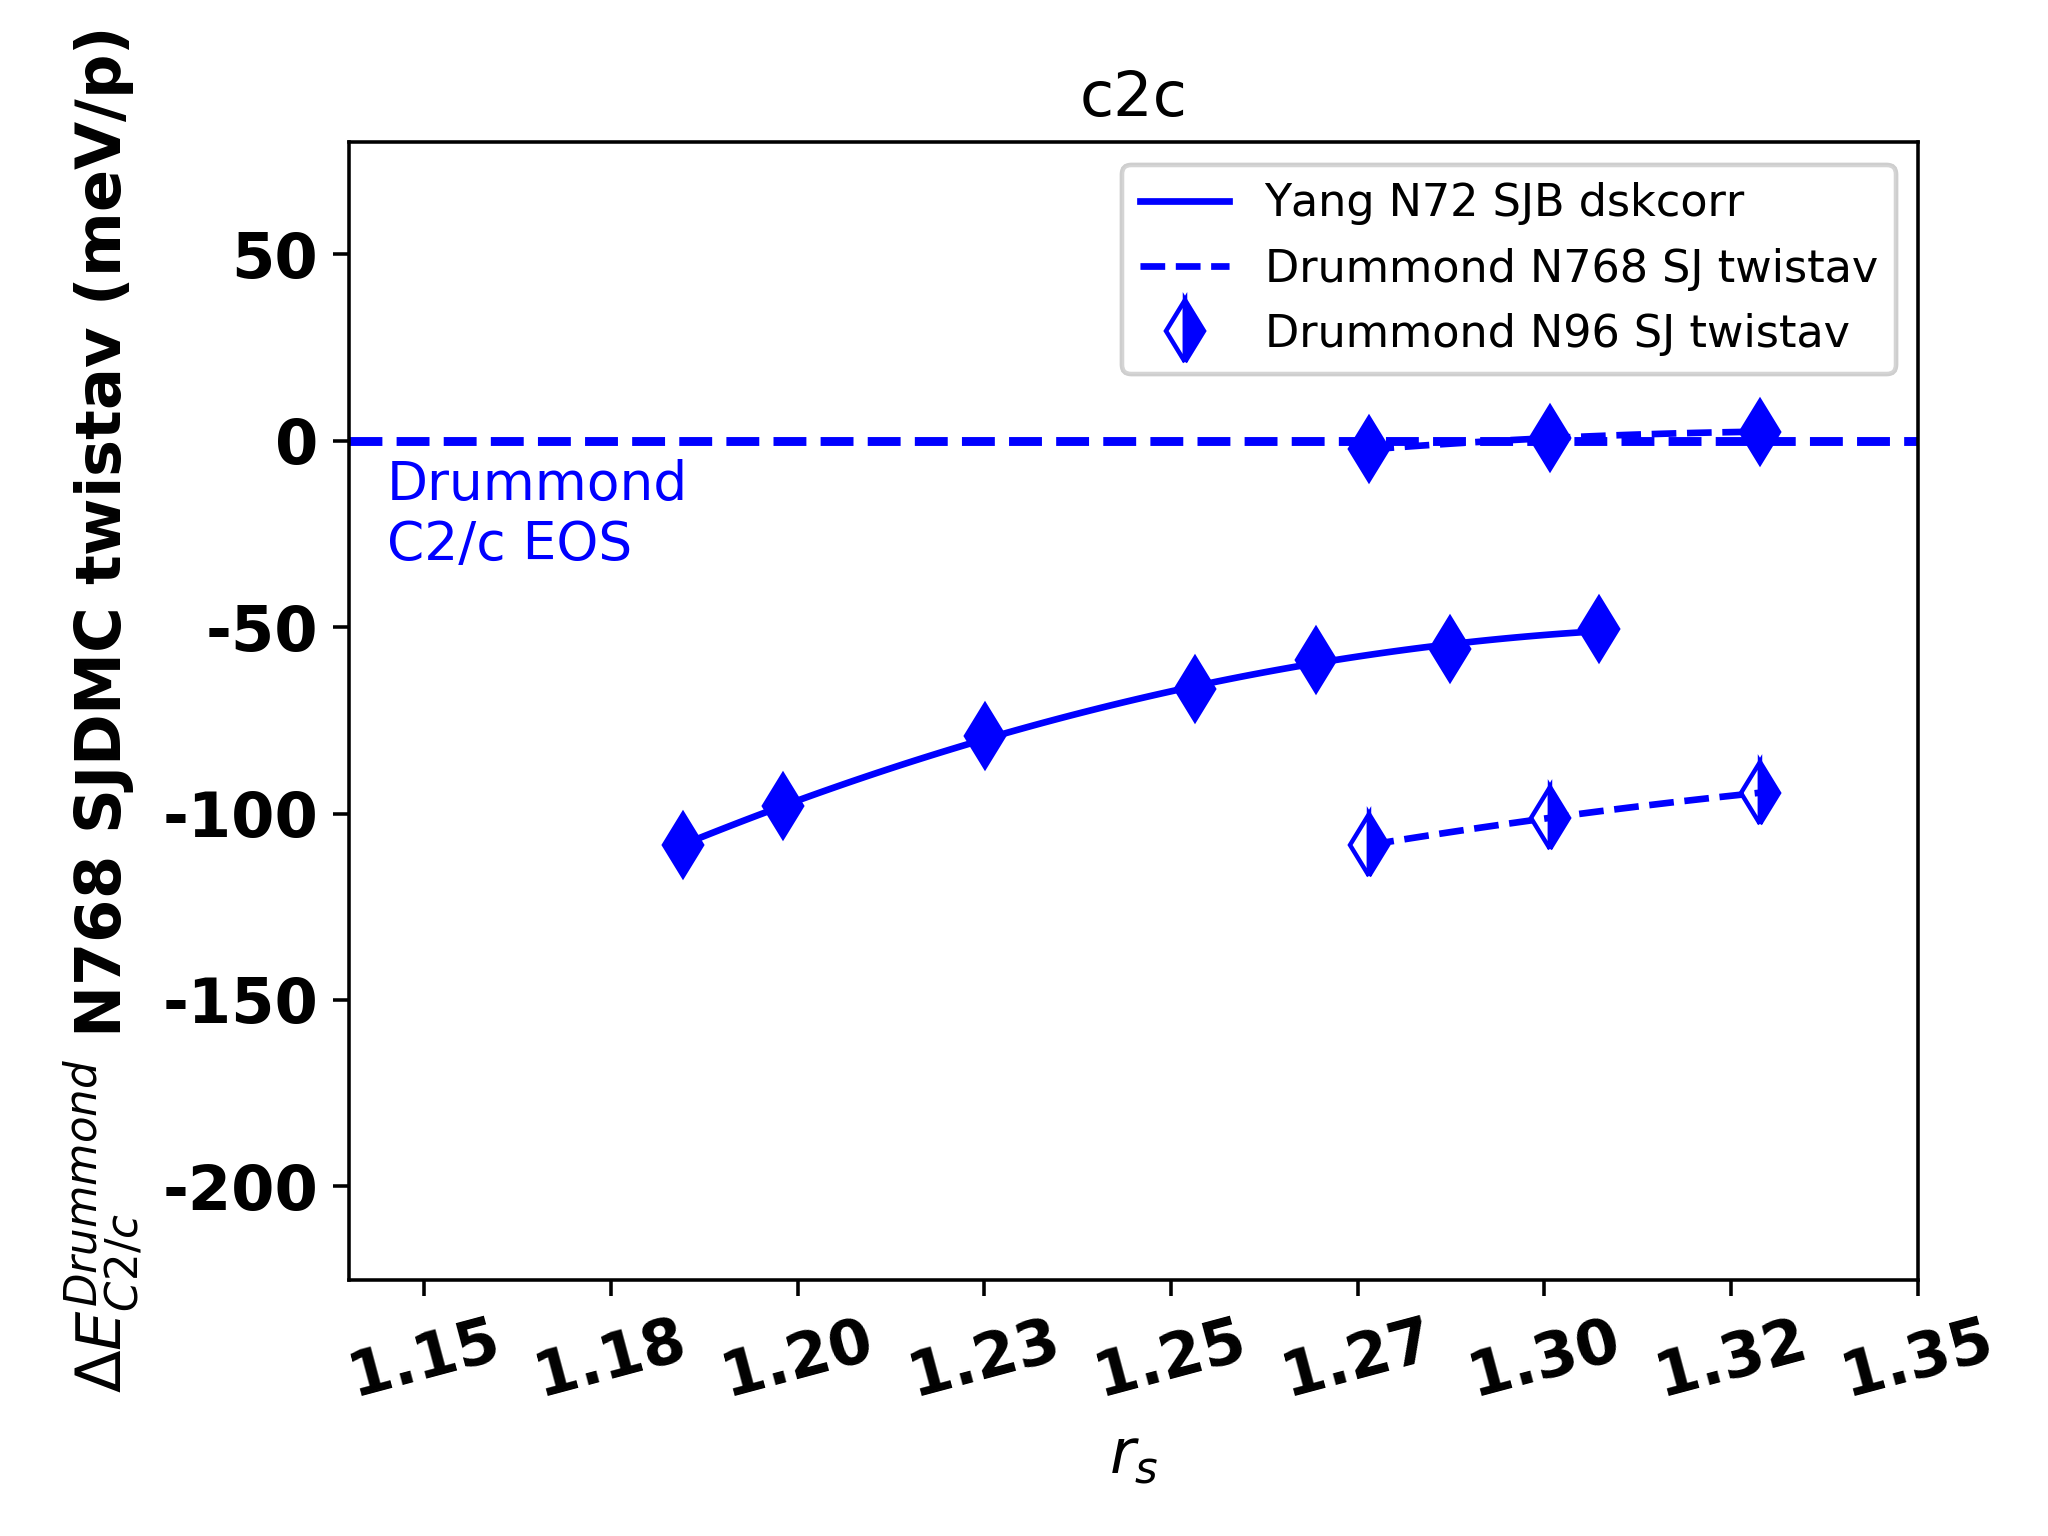
\includegraphics[scale=0.48]{006b_c2c_step0}
(a) DMC data.%\label{fig:static-c2c-yang-drummond-data}
\end{minipage}
%\begin{subfigure}{0.48\textwidth}
%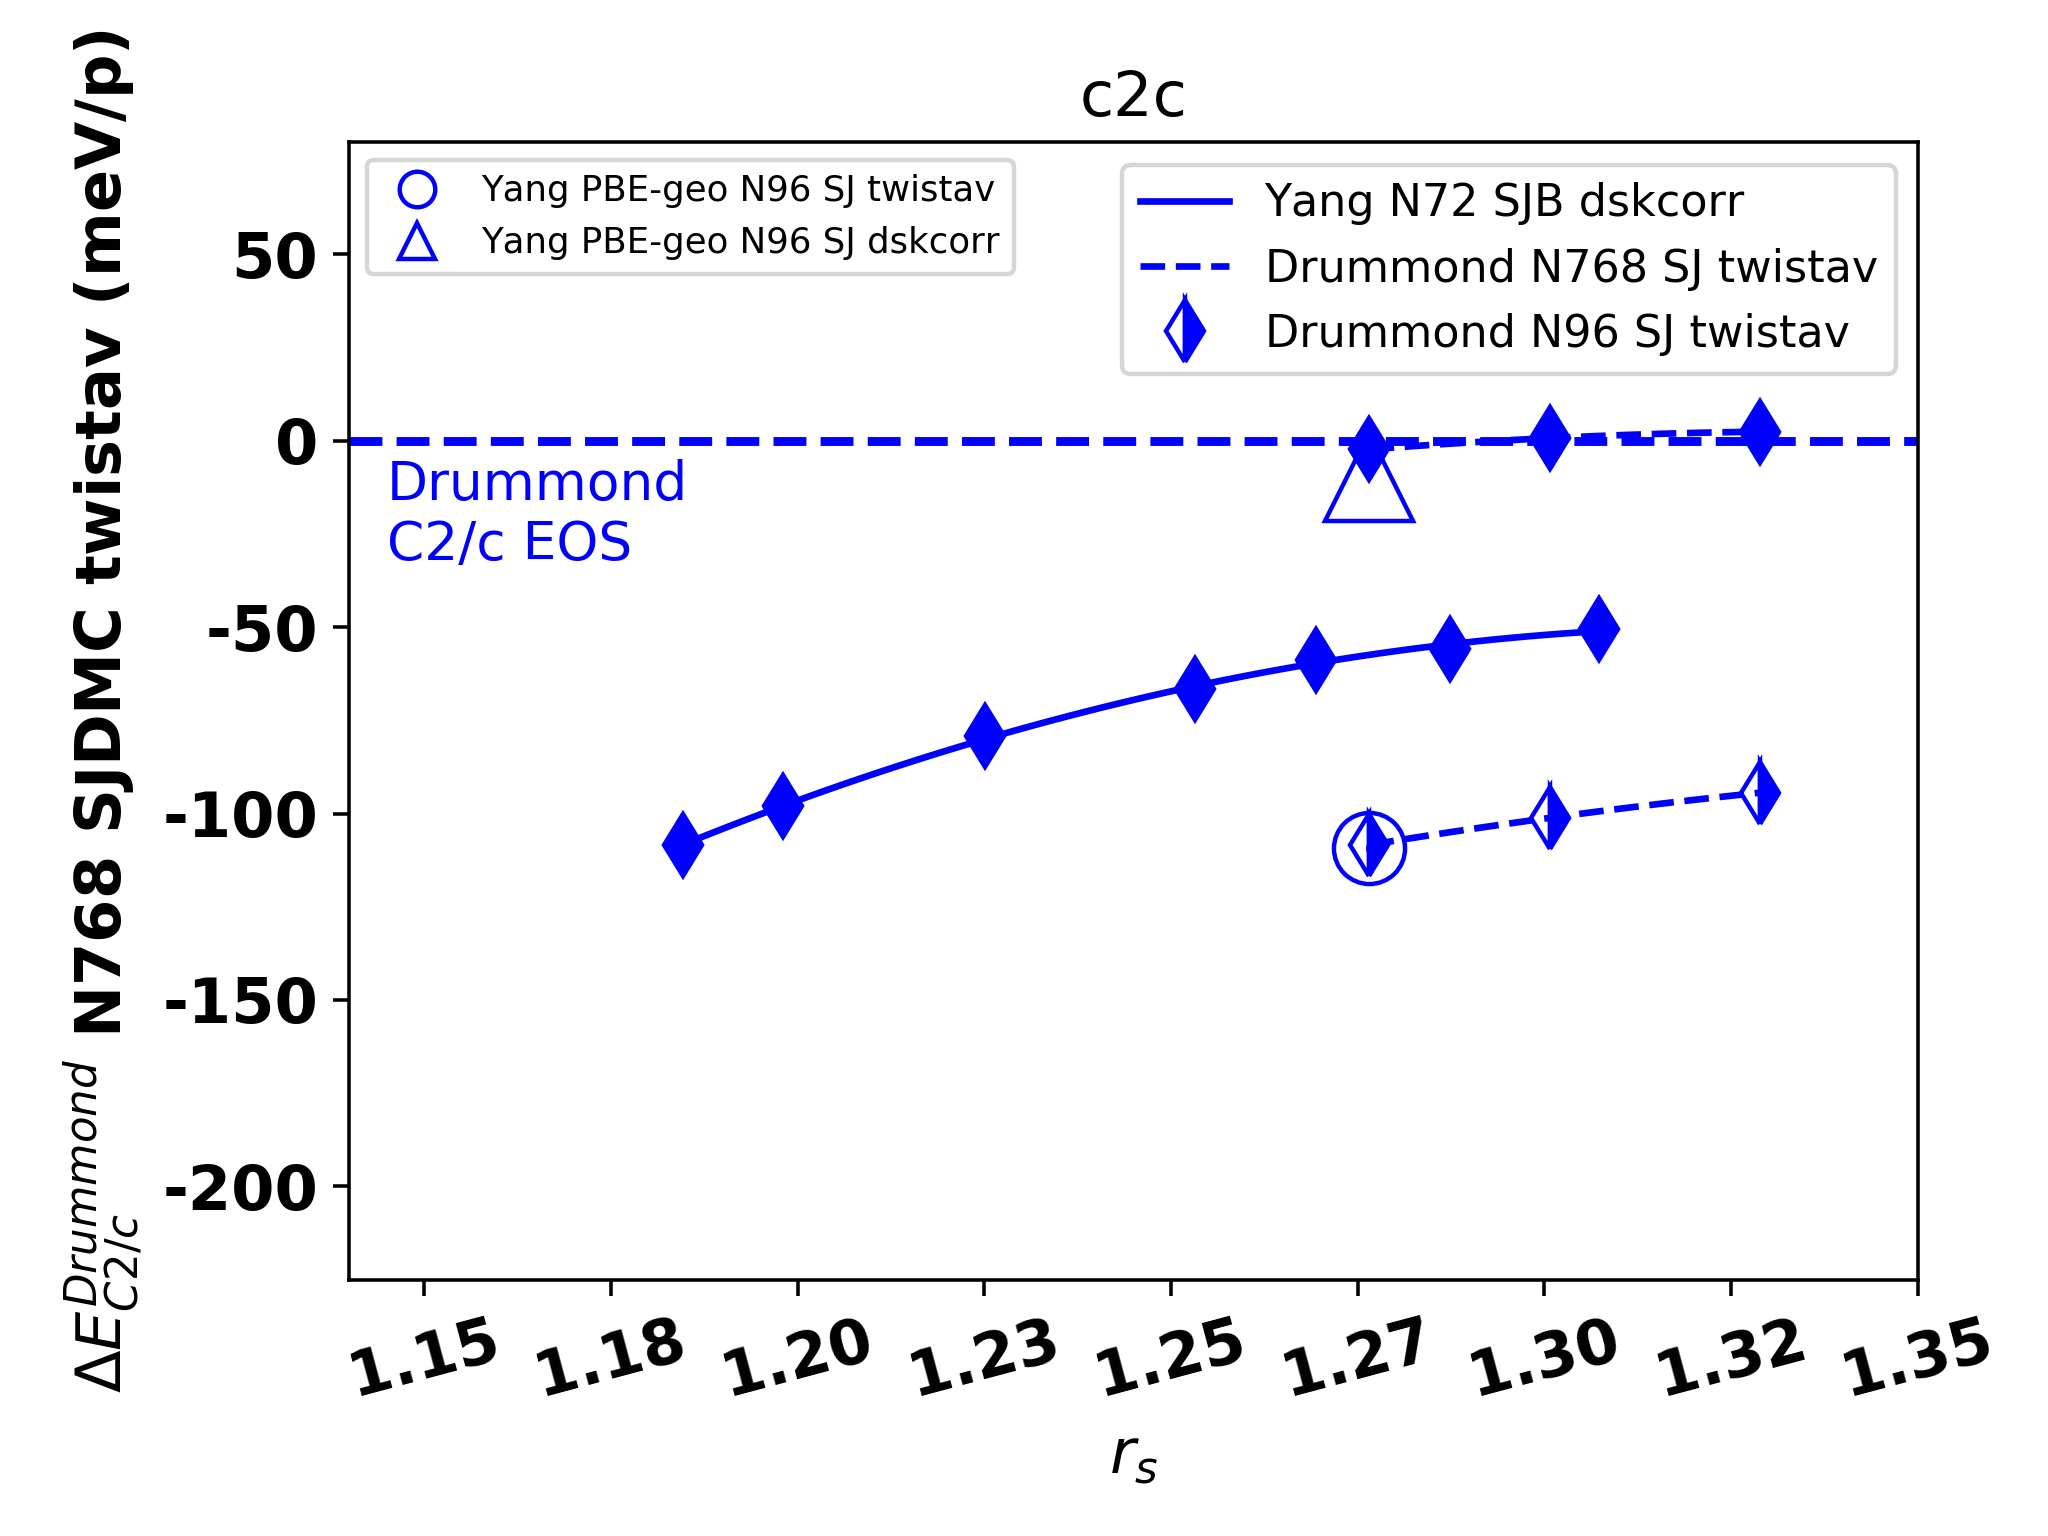
\includegraphics[scale=0.48]{figures/c2c/006b_c2c_step2}
%\caption{Reproduce PBE-geo N768 SJ twistav.\label{fig:static-c2c-yang-drummond-fs}}
%\end{subfigure}
%\begin{subfigure}{0.48\textwidth}
%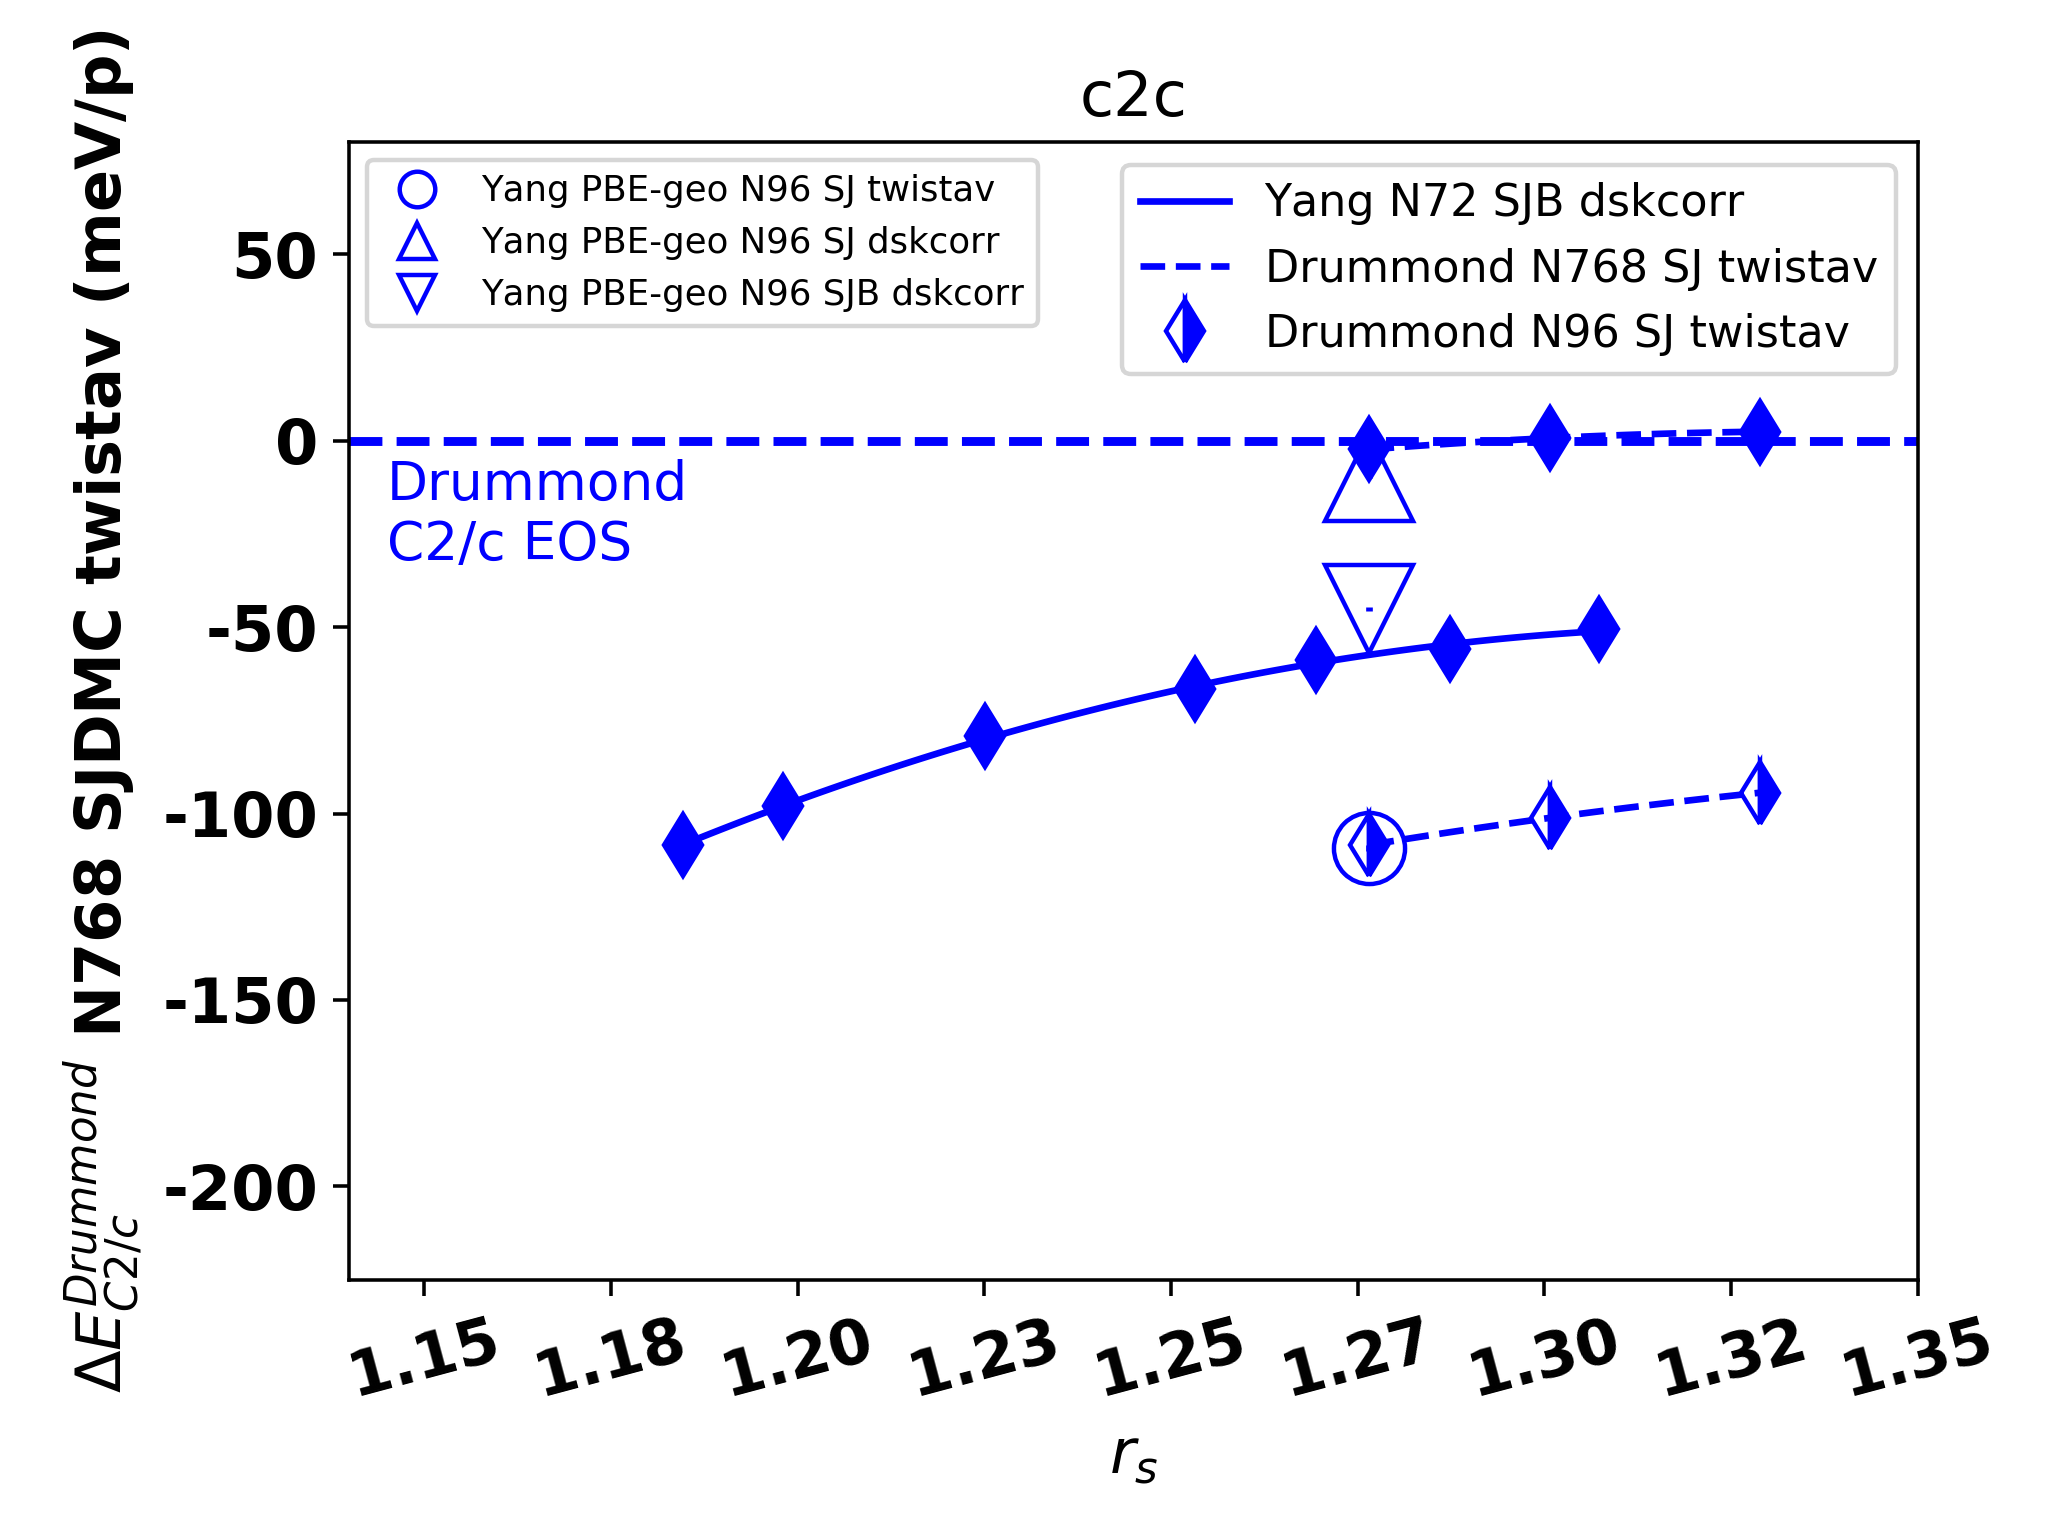
\includegraphics[scale=0.48]{figures/c2c/006b_c2c_step3}
%\caption{Effect of backflow.\label{fig:static-c2c-yang-drummond-bf}}
%\end{subfigure}
%\begin{subfigure}{0.48\textwidth}
%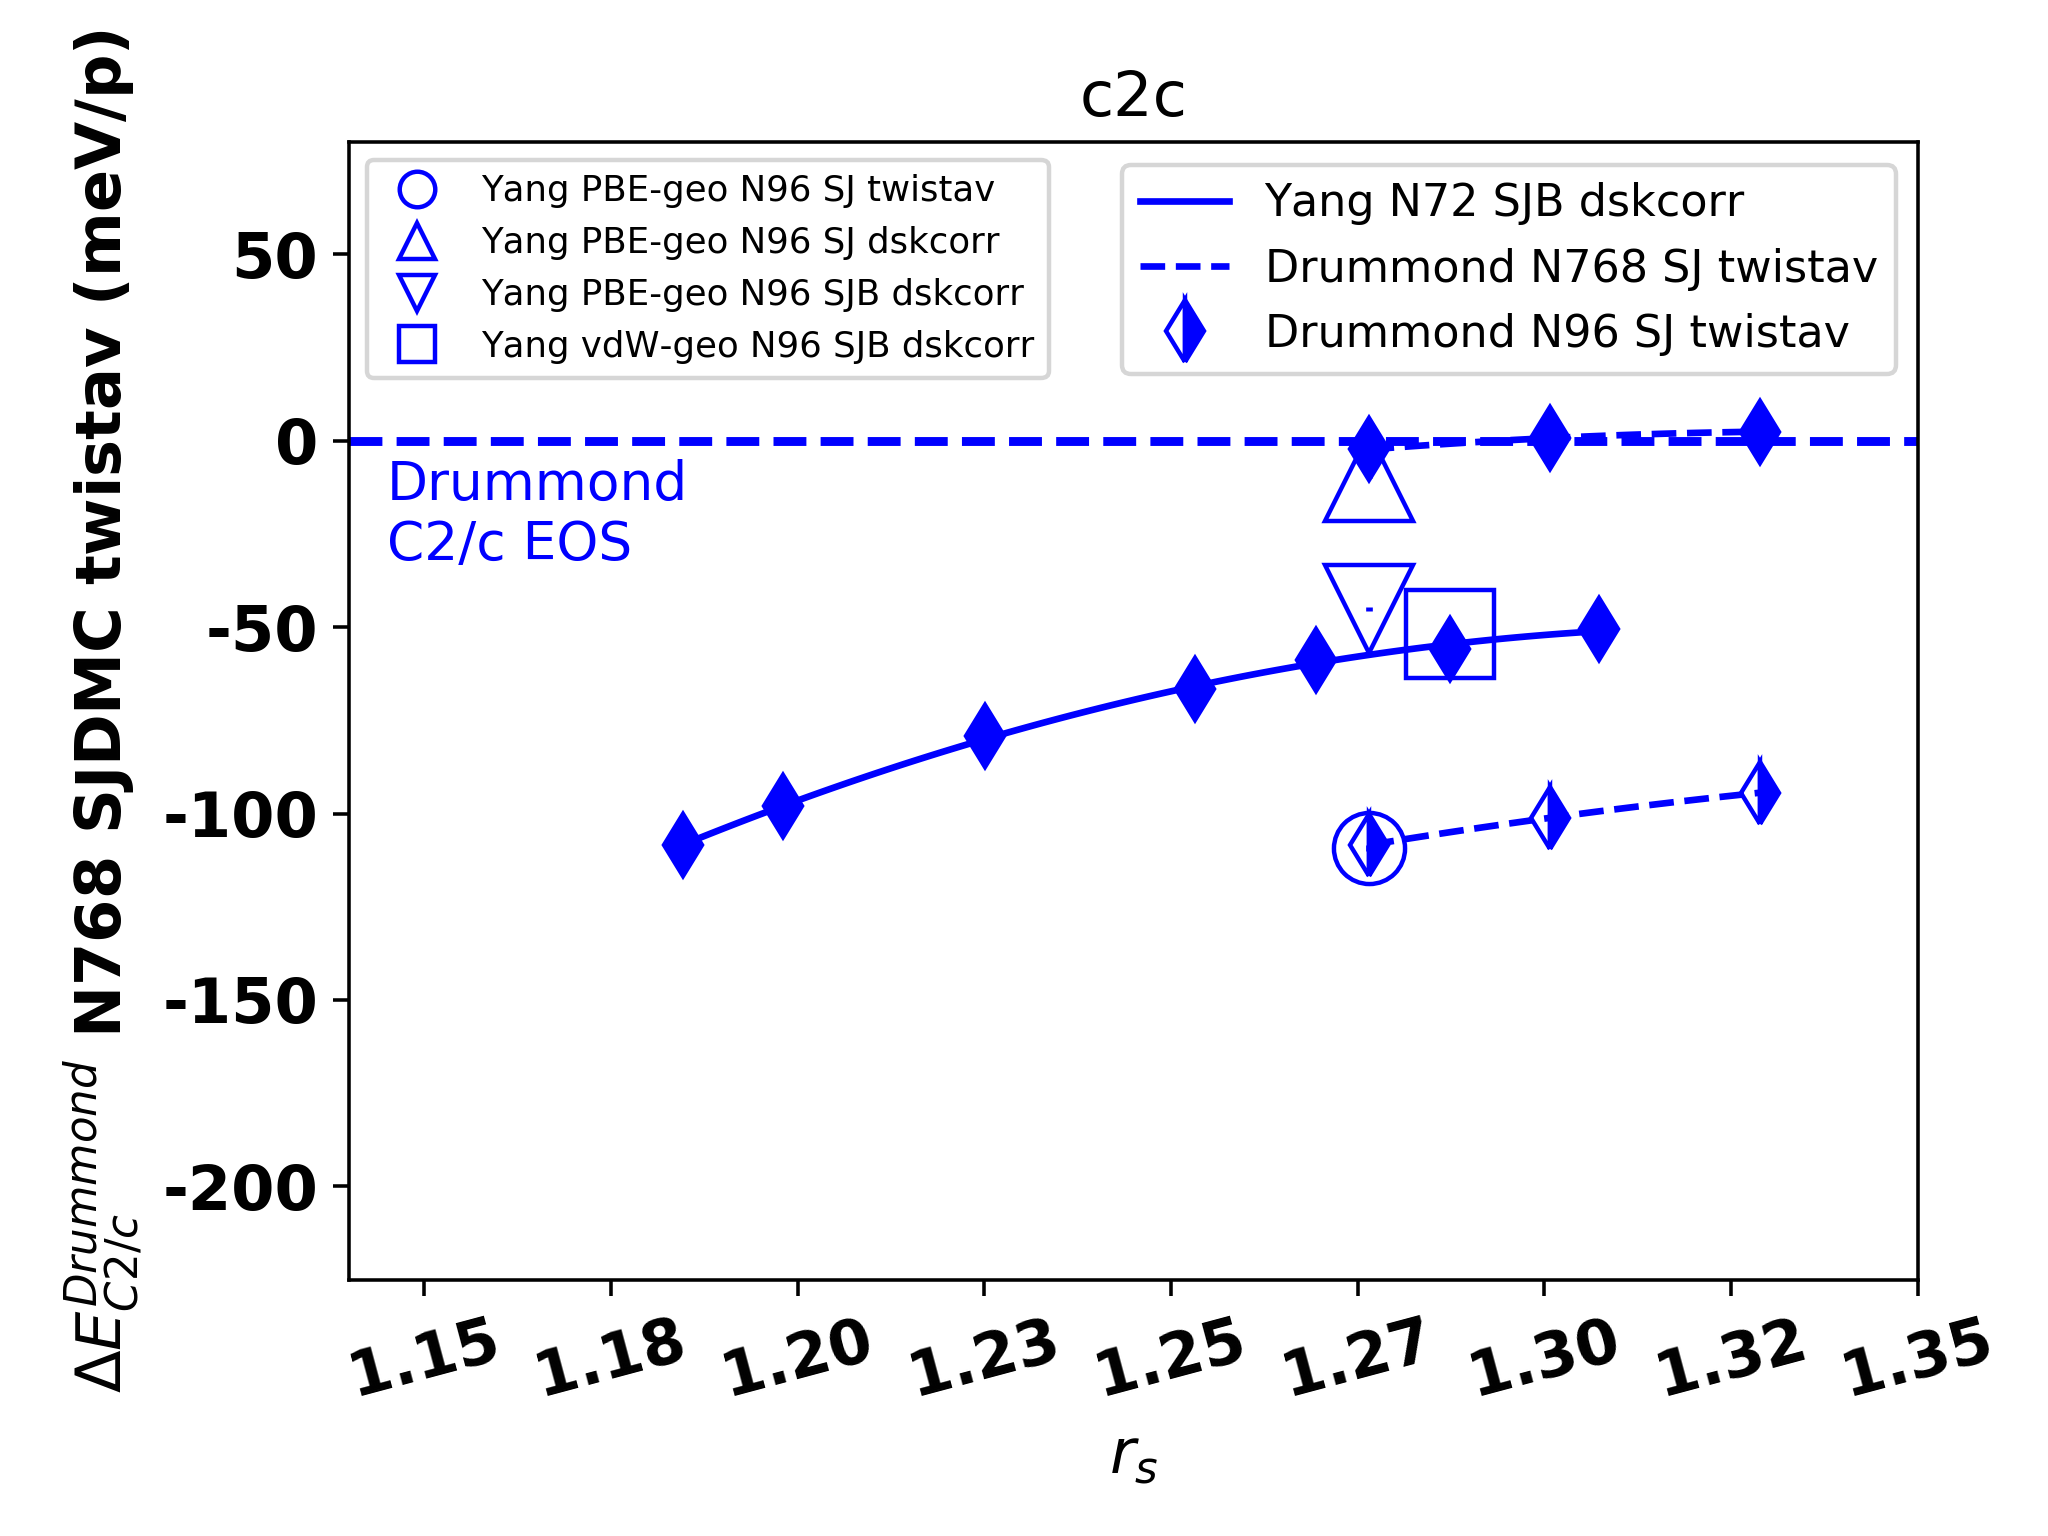
\includegraphics[scale=0.48]{figures/c2c/006b_c2c_step4}
%\caption{Effect of vdW-geo.\label{fig:static-c2c-yang-drummond-geo}}
%\end{subfigure}
\begin{minipage}{0.48\textwidth}
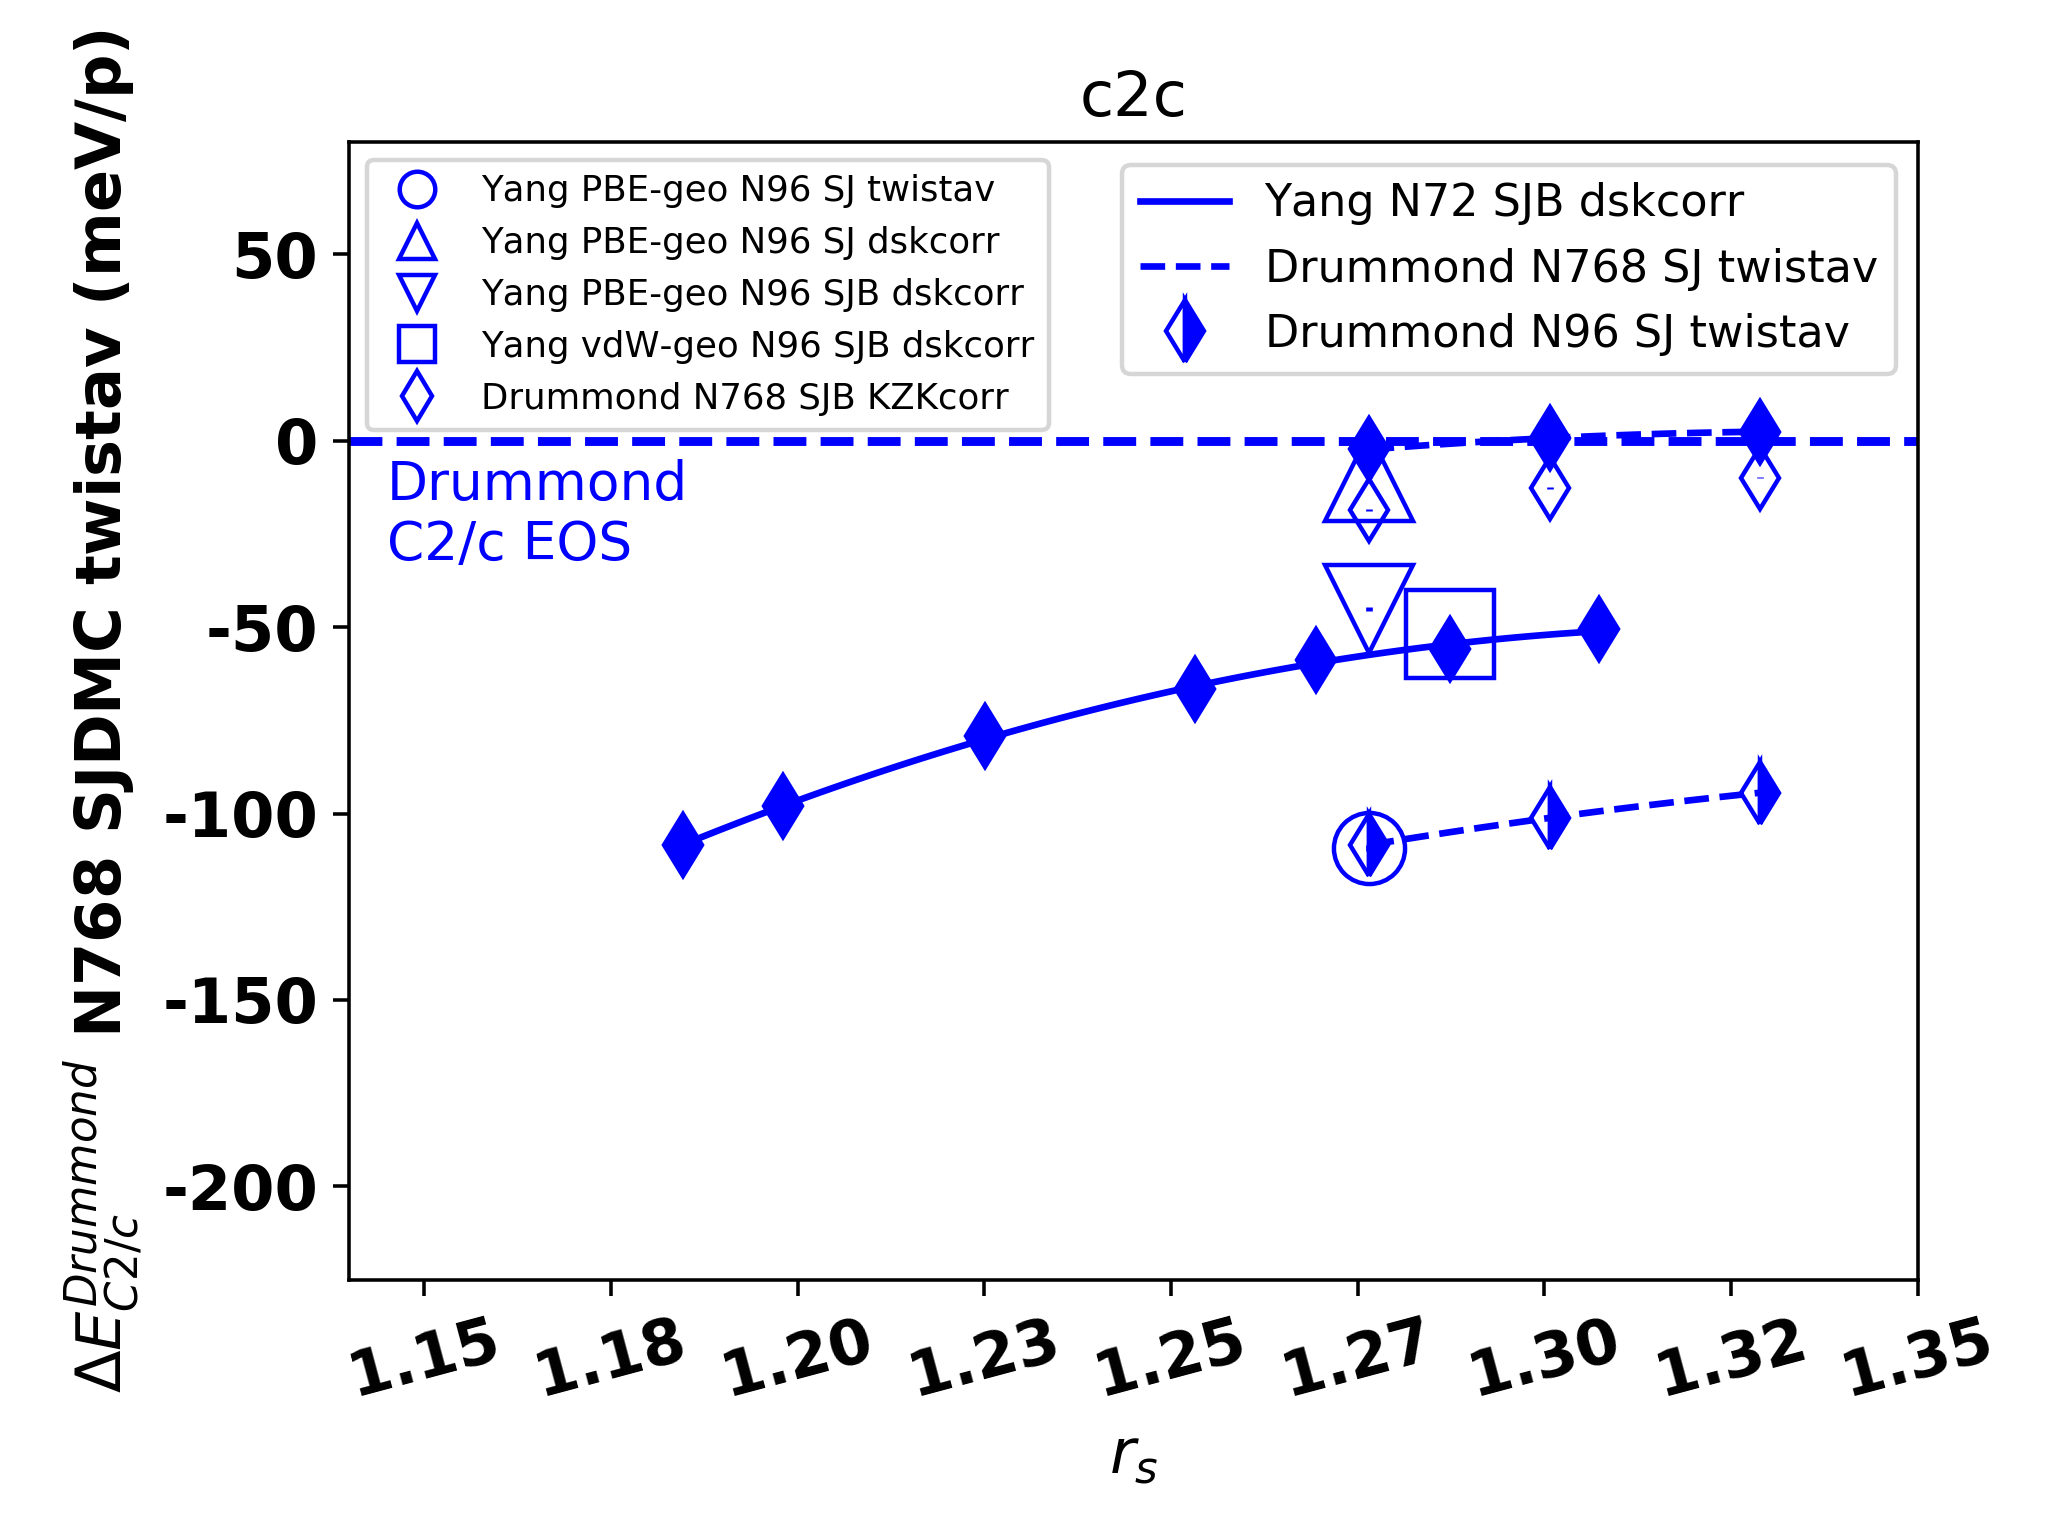
\includegraphics[scale=0.48]{006b_c2c_step5}
(b) Drummond SJB. %\label{fig:static-c2c-yang-drummond-last}
\end{minipage}
\caption{C2/c-24 DMC total energy relative to reference EOS.\label{fig:static-c2c-yang-drummond}}
\end{figure}

\subsection{Atomic Phase Candidate I4$_1$/amd}

Four sets of data are shown in Fig.~\ref{fig:static-i41amd-yang-mcminis-azadi}. A series of calculations are added in Fig.~\ref{fig:static-i41amd-yang-mcminis-azadi-data}-\ref{fig:static-i41amd-yang-mcminis-azadi-last} to connect them. Phase III EOS eqn.~\ref{eq:drum_sjdmc_n768} is again used as reference. The solid stars connected by a dot-dashed line are McMinis' SJ results. The solid stars connected by a dotted line are Azadi's FS-corrected results. The solid stars connected by a solid line are my results. Finally, the right-filled starts connected by dot-dashed lines are Azadi's N128 SJB twistav results without the Chiesa correction.

In Fig.~\ref{fig:static-i41amd-yang-mcminis-azadi-repro}, I attempt to reproduce Azadi's 128-atom results using QMCPACK (open stars). At $r_s=1.25$, our energies agree within 3 sigmas. However, at $r_s=1.17$, my energy is 18 meV/p higher than Azadi's. In Fig.~\ref{fig:static-i41amd-yang-mcminis-azadi-fs}, I add dskcorr to previous simulations and reproduce my N72 SJB energies (open downward triangles). In Fig.~\ref{fig:static-i41amd-yang-mcminis-azadi-last}, I remove back flow from previous simulations and obtain energies close to McMinis' results. At $r_s=1.17$, my N128 SJ dskcorr energy is 8(2) meV/p lower than McMinis'.

The difference between my N72 SJ dskcorr and McMinis' Ninf SJ energy is 8 meV/p. Assuming McMinis' energies are the correct thermodynamic values, then the remaining FS error after dskcorr is 8 meV/p. This is much lower than the remaining FS error in the molecular structures. Further, comparing the upward open triangles (SJ) and the downward open triangles (SJB), we see that back flow transformation gains $\sim$40 meV/p. Indeed, after shifting McMinis' energies by 48 meV/p (1.8 mha/p), our results agree well (Fig.~\ref{fig:static-enthalpy-vs-pressure}).

The 18 meV/p energy difference between mine and Azadi's twistav energies cannot be satisfactorily explained. Azadi used a different atomic structures than McMinis and myself. However, the energy variation caused by the structure difference should be no more than 5 meV/p.

%\begin{figure}[h]
%\begin{subfigure}{0.48\textwidth}
%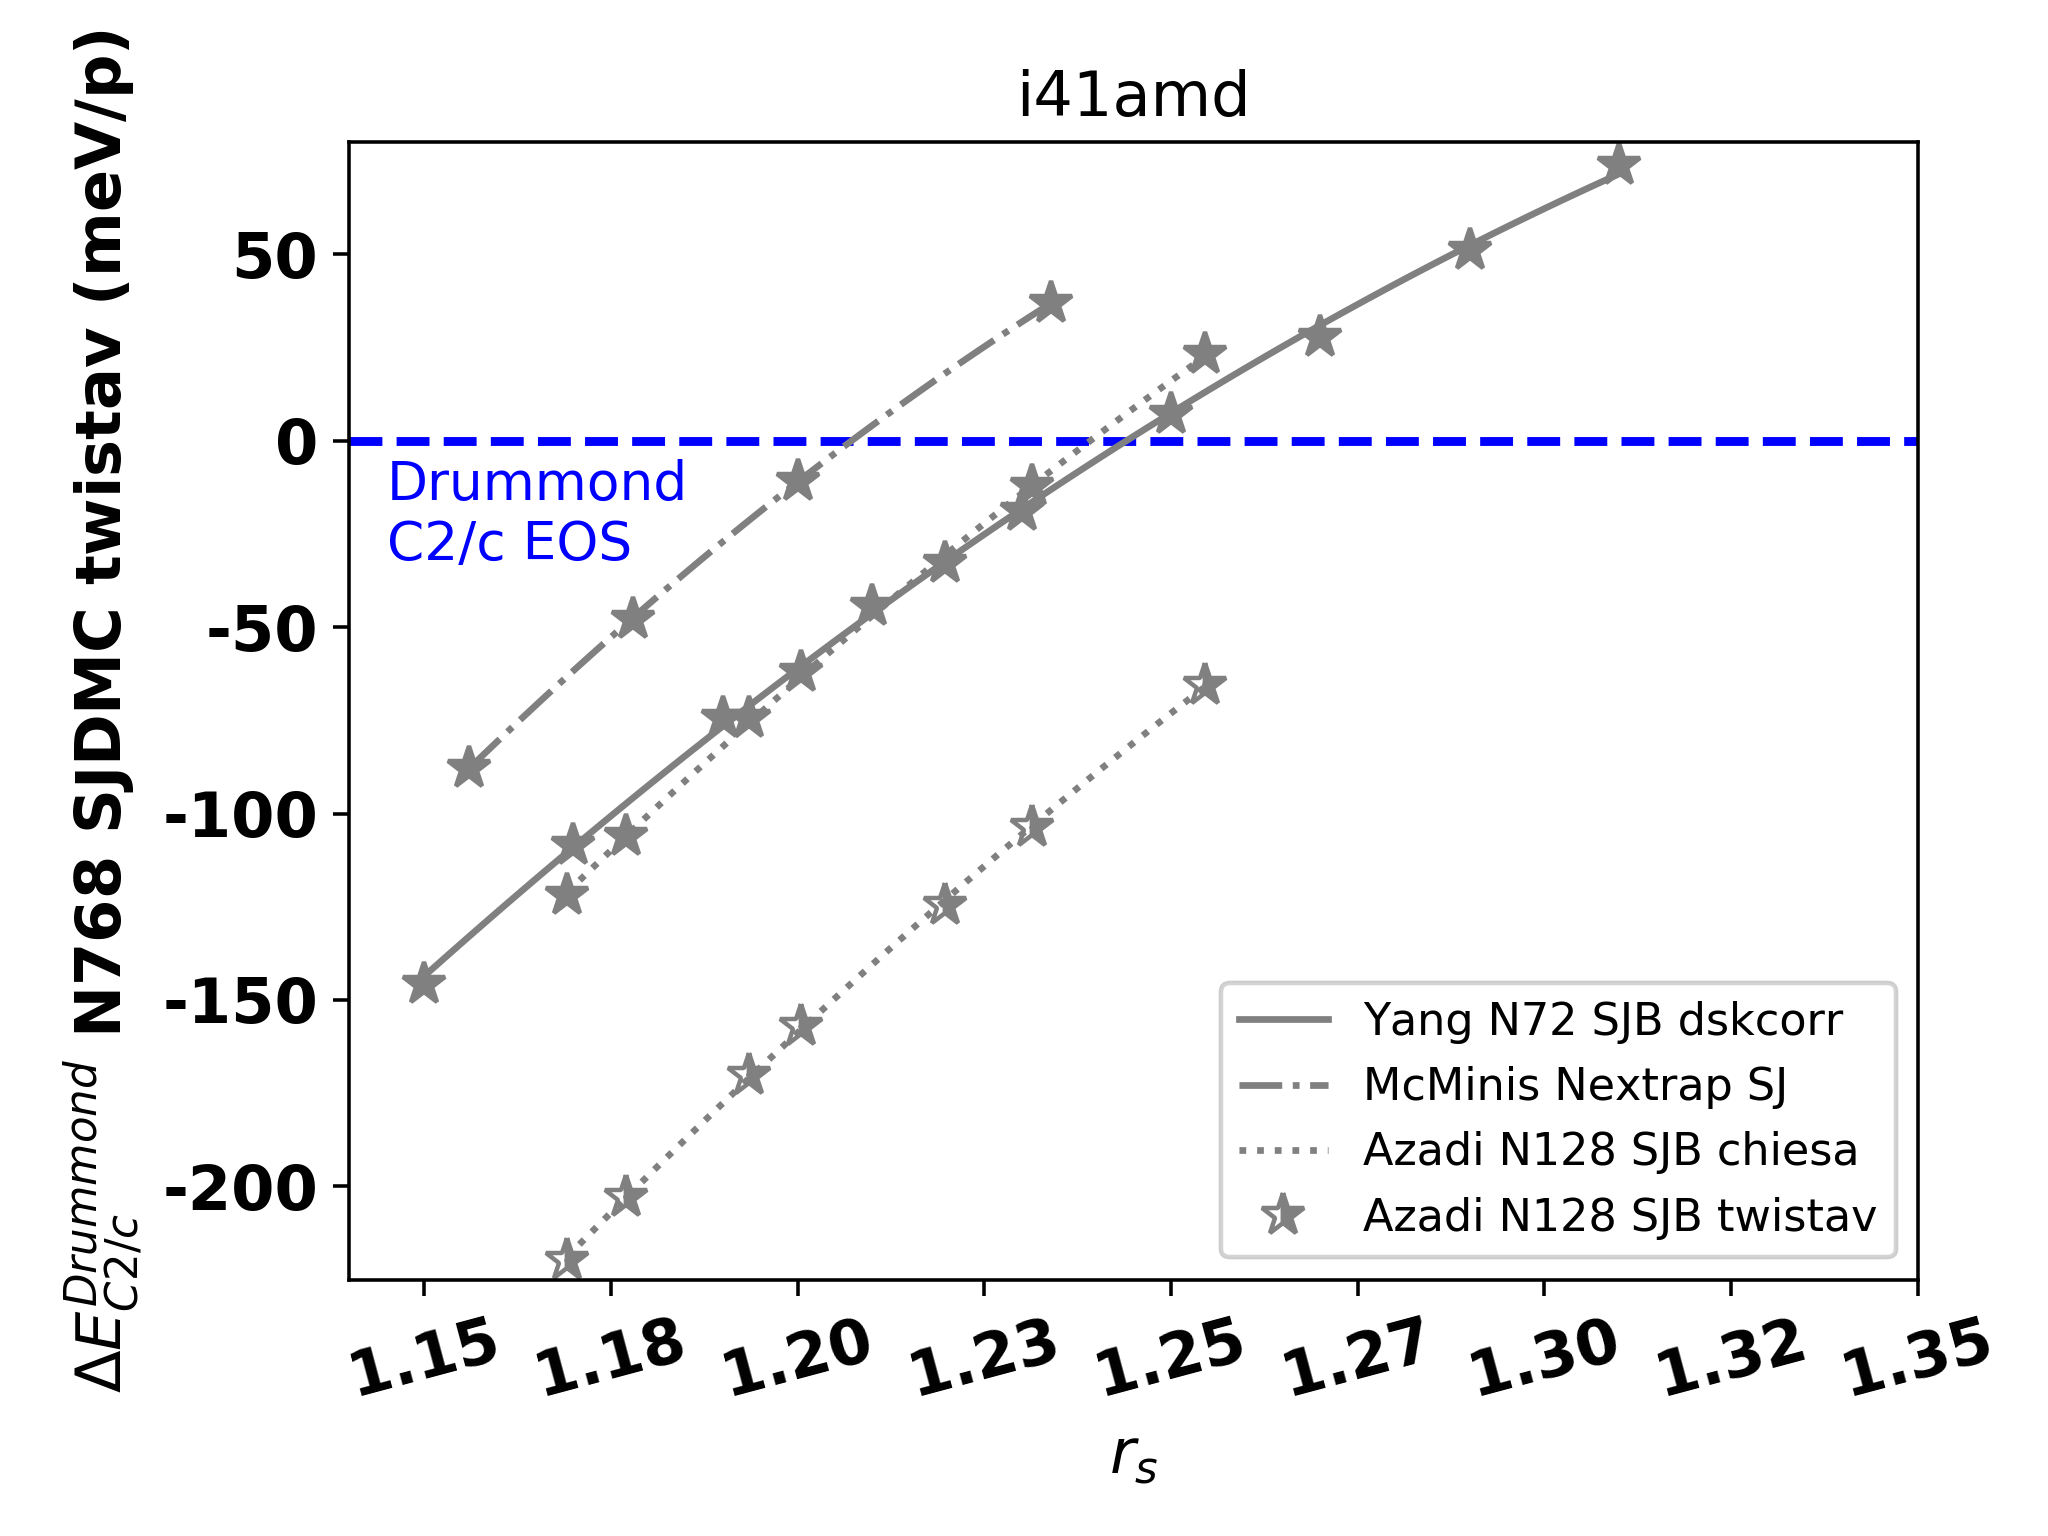
\includegraphics[scale=0.48]{figures/i41amd/006b_i41amd_step0}
%\caption{DMC data.\label{fig:static-i41amd-yang-mcminis-azadi-data}}
%\end{subfigure}
%\begin{subfigure}{0.48\textwidth}
%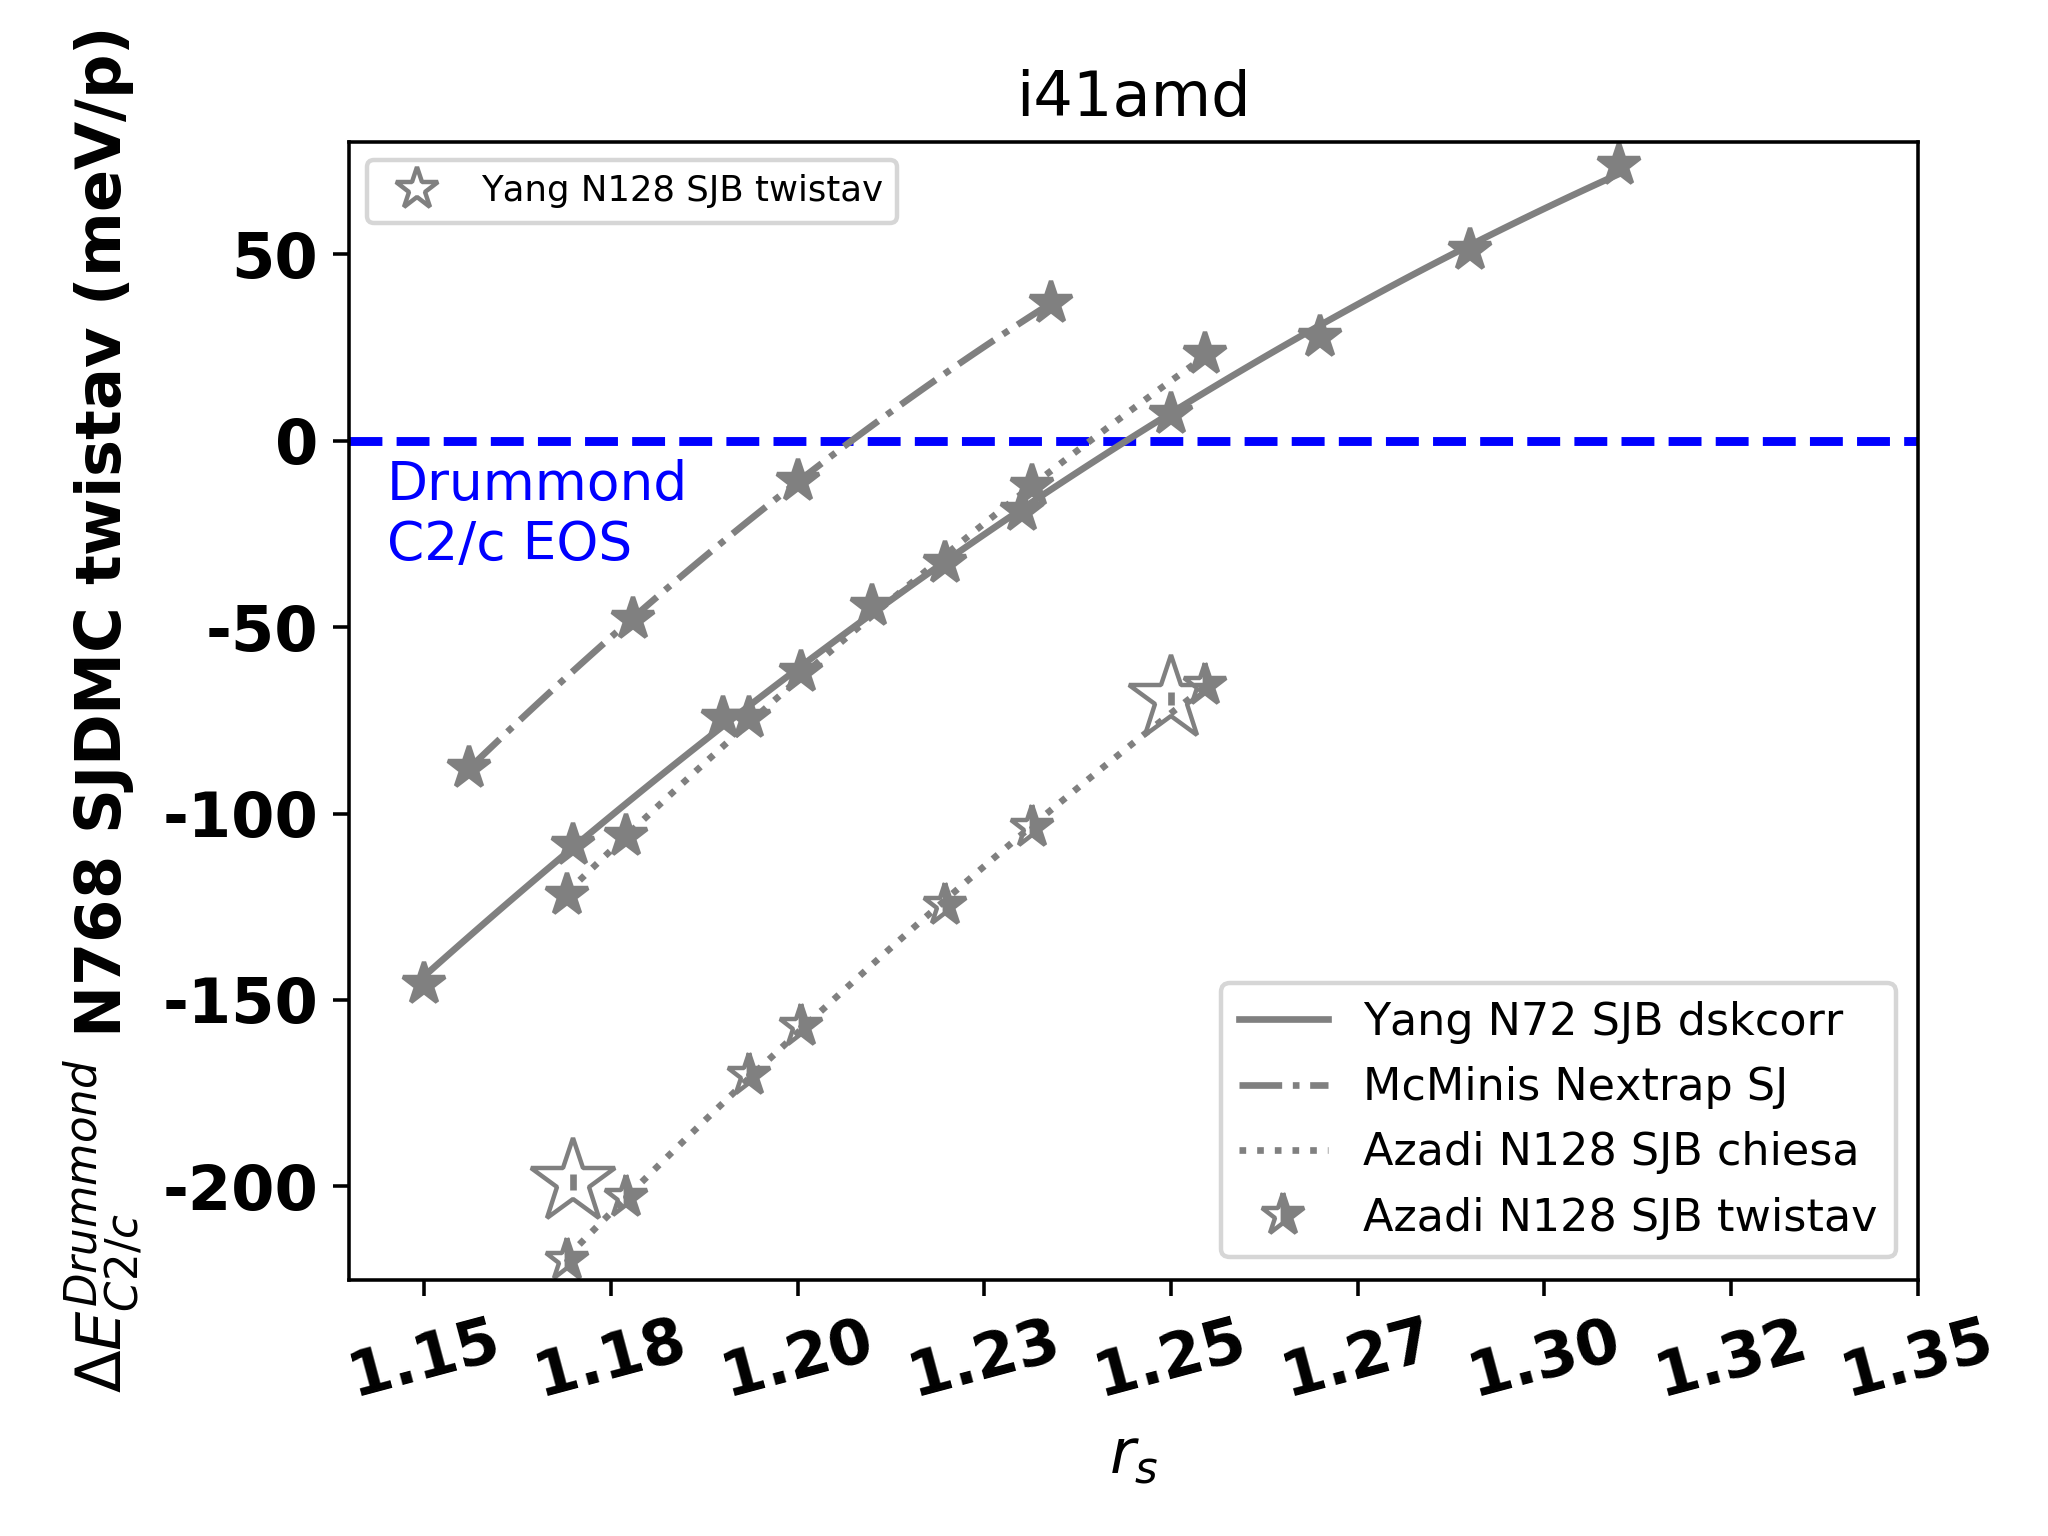
\includegraphics[scale=0.48]{figures/i41amd/006b_i41amd_step1}
%\caption{Reproduce PBE-geo N128 SJB twistav.\label{fig:static-i41amd-yang-mcminis-azadi-repro}}
%\end{subfigure}
%\begin{subfigure}{0.48\textwidth}
%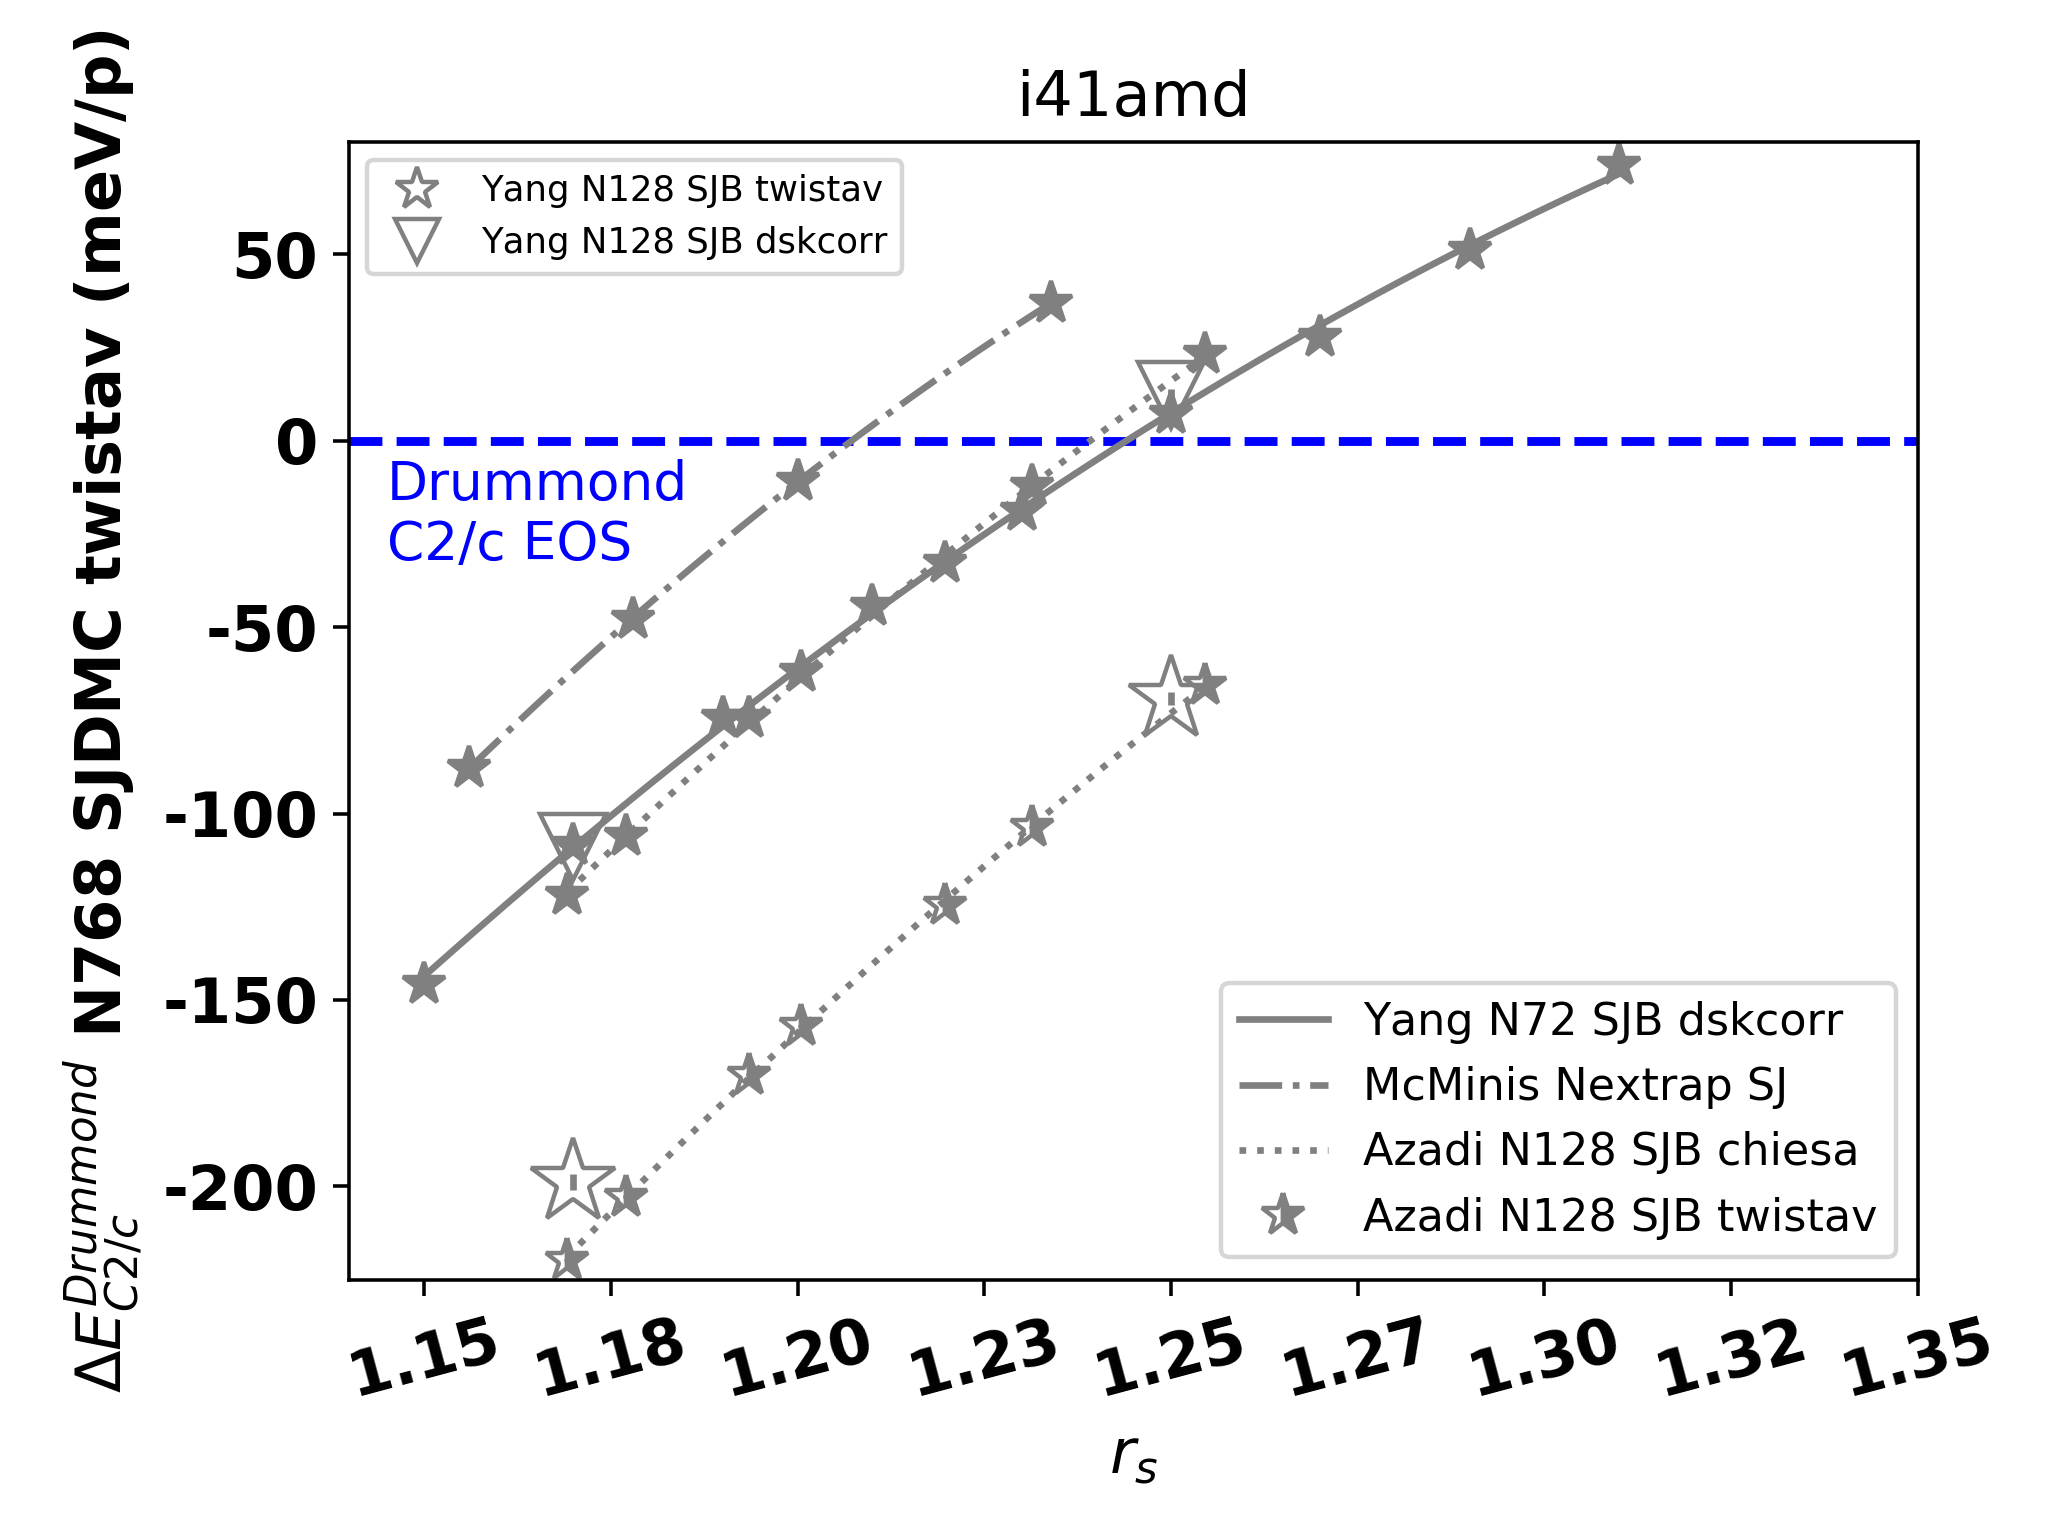
\includegraphics[scale=0.48]{figures/i41amd/006b_i41amd_step2}
%\caption{Match N96 and N72 using dskcorr.\label{fig:static-i41amd-yang-mcminis-azadi-fs}}
%\end{subfigure}
%\begin{subfigure}{0.48\textwidth}
%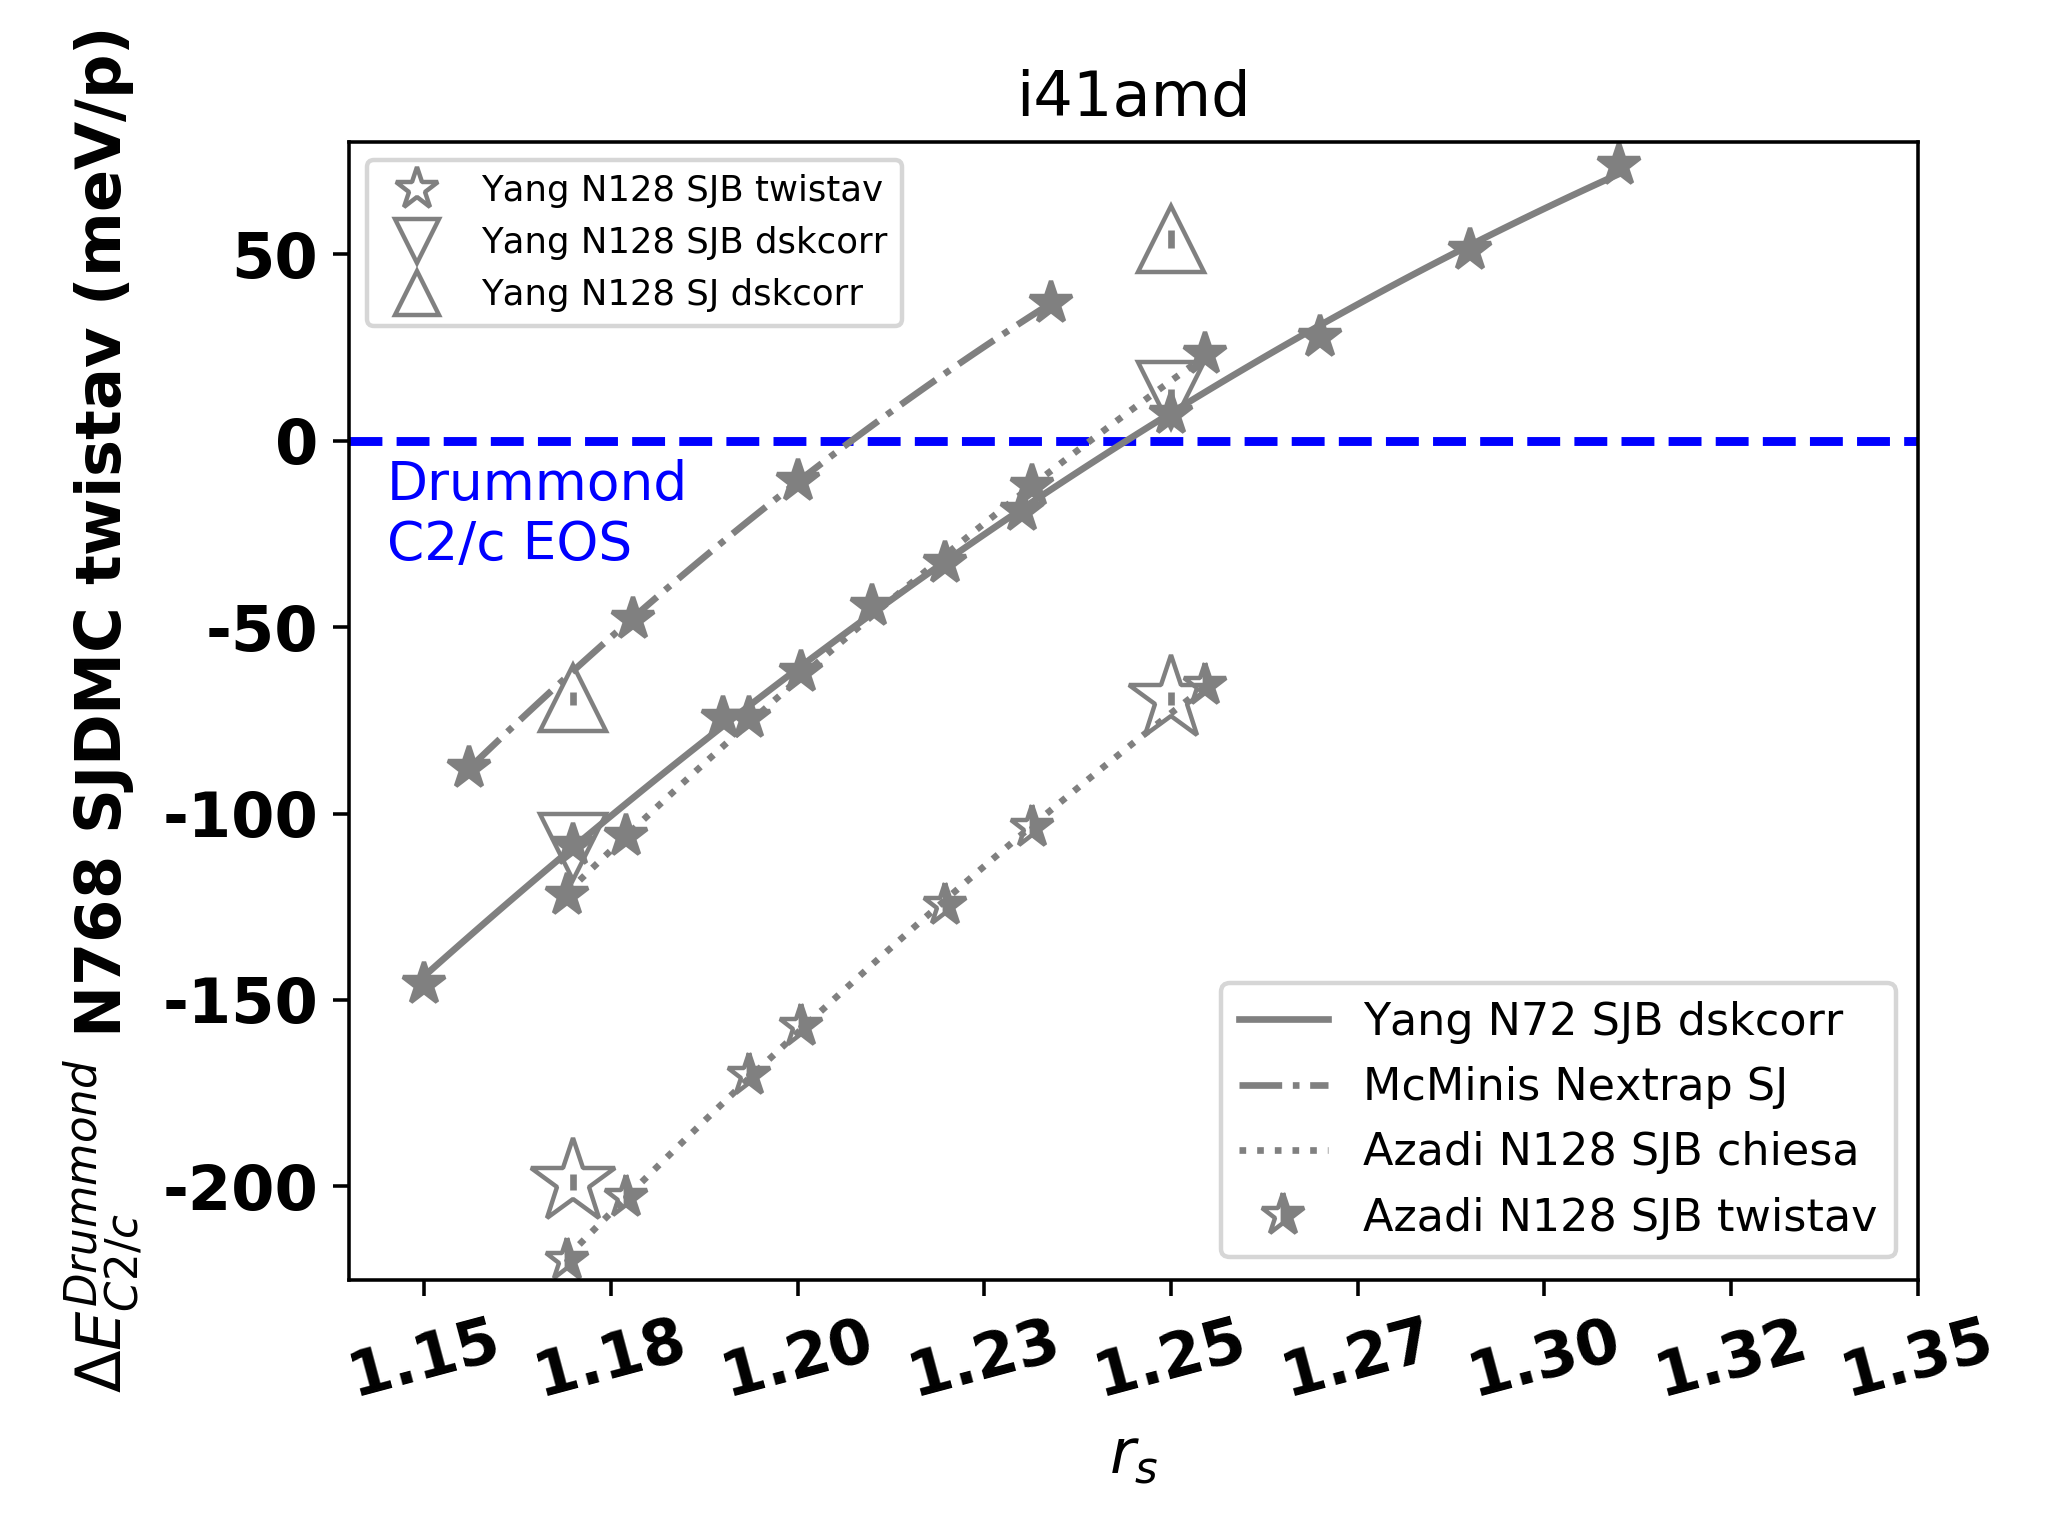
\includegraphics[scale=0.48]{figures/i41amd/006b_i41amd_step3}
%\caption{Reproduce McMinis SJ.\label{fig:static-i41amd-yang-mcminis-azadi-last}}
%\end{subfigure}
%\caption{I4$_1$/amd\label{fig:static-i41amd-yang-mcminis-azadi}}
%\end{figure}

\subsection{Molecular Candidate Cmca-4}

Three sets of data are shown in Fig.~\ref{fig:static-cmca4-yang-drummond-azadi}. The same reference EOS eq.~(\ref{eq:drum_sjdmc_n768}) is used as before. The solid downward triangles connected by a dashed line are Drummond N768 SJ twistav results. The solid downward triangles connected by a dotted line are Azadi's N128 SJB chiesa results [Azadi2014SI]. Finally, the solid downward triangles connected by a solid line are my N72 SJB dskcorr results.

In Fig.~\ref{fig:static-cmca4-yang-drummond-azadi-kzk}, KZKcorr=13-14 meV/p is added to Drummond SJ results to produce the top-filled downward triangles. In Fig.~\ref{fig:static-cmca4-yang-drummond-azadi-sjb}, Drummond's back flow results, corrected by KZKcorr, are shown as open downward triangles. At $r_s=1.30$ my SBJ dskcorr energy is lower than Drummond's SBJ KZKcorr energy by \textbf{37 meV/p}.

Azadi's SJB results are more consistent with Drummond's SJ results than SJB results. This discrepancy is unlikely to be due to the Chiesa correction because the remaining FS error after the Chiesa correction is usually negative.

\begin{figure}[h]
\begin{minipage}{0.48\textwidth}
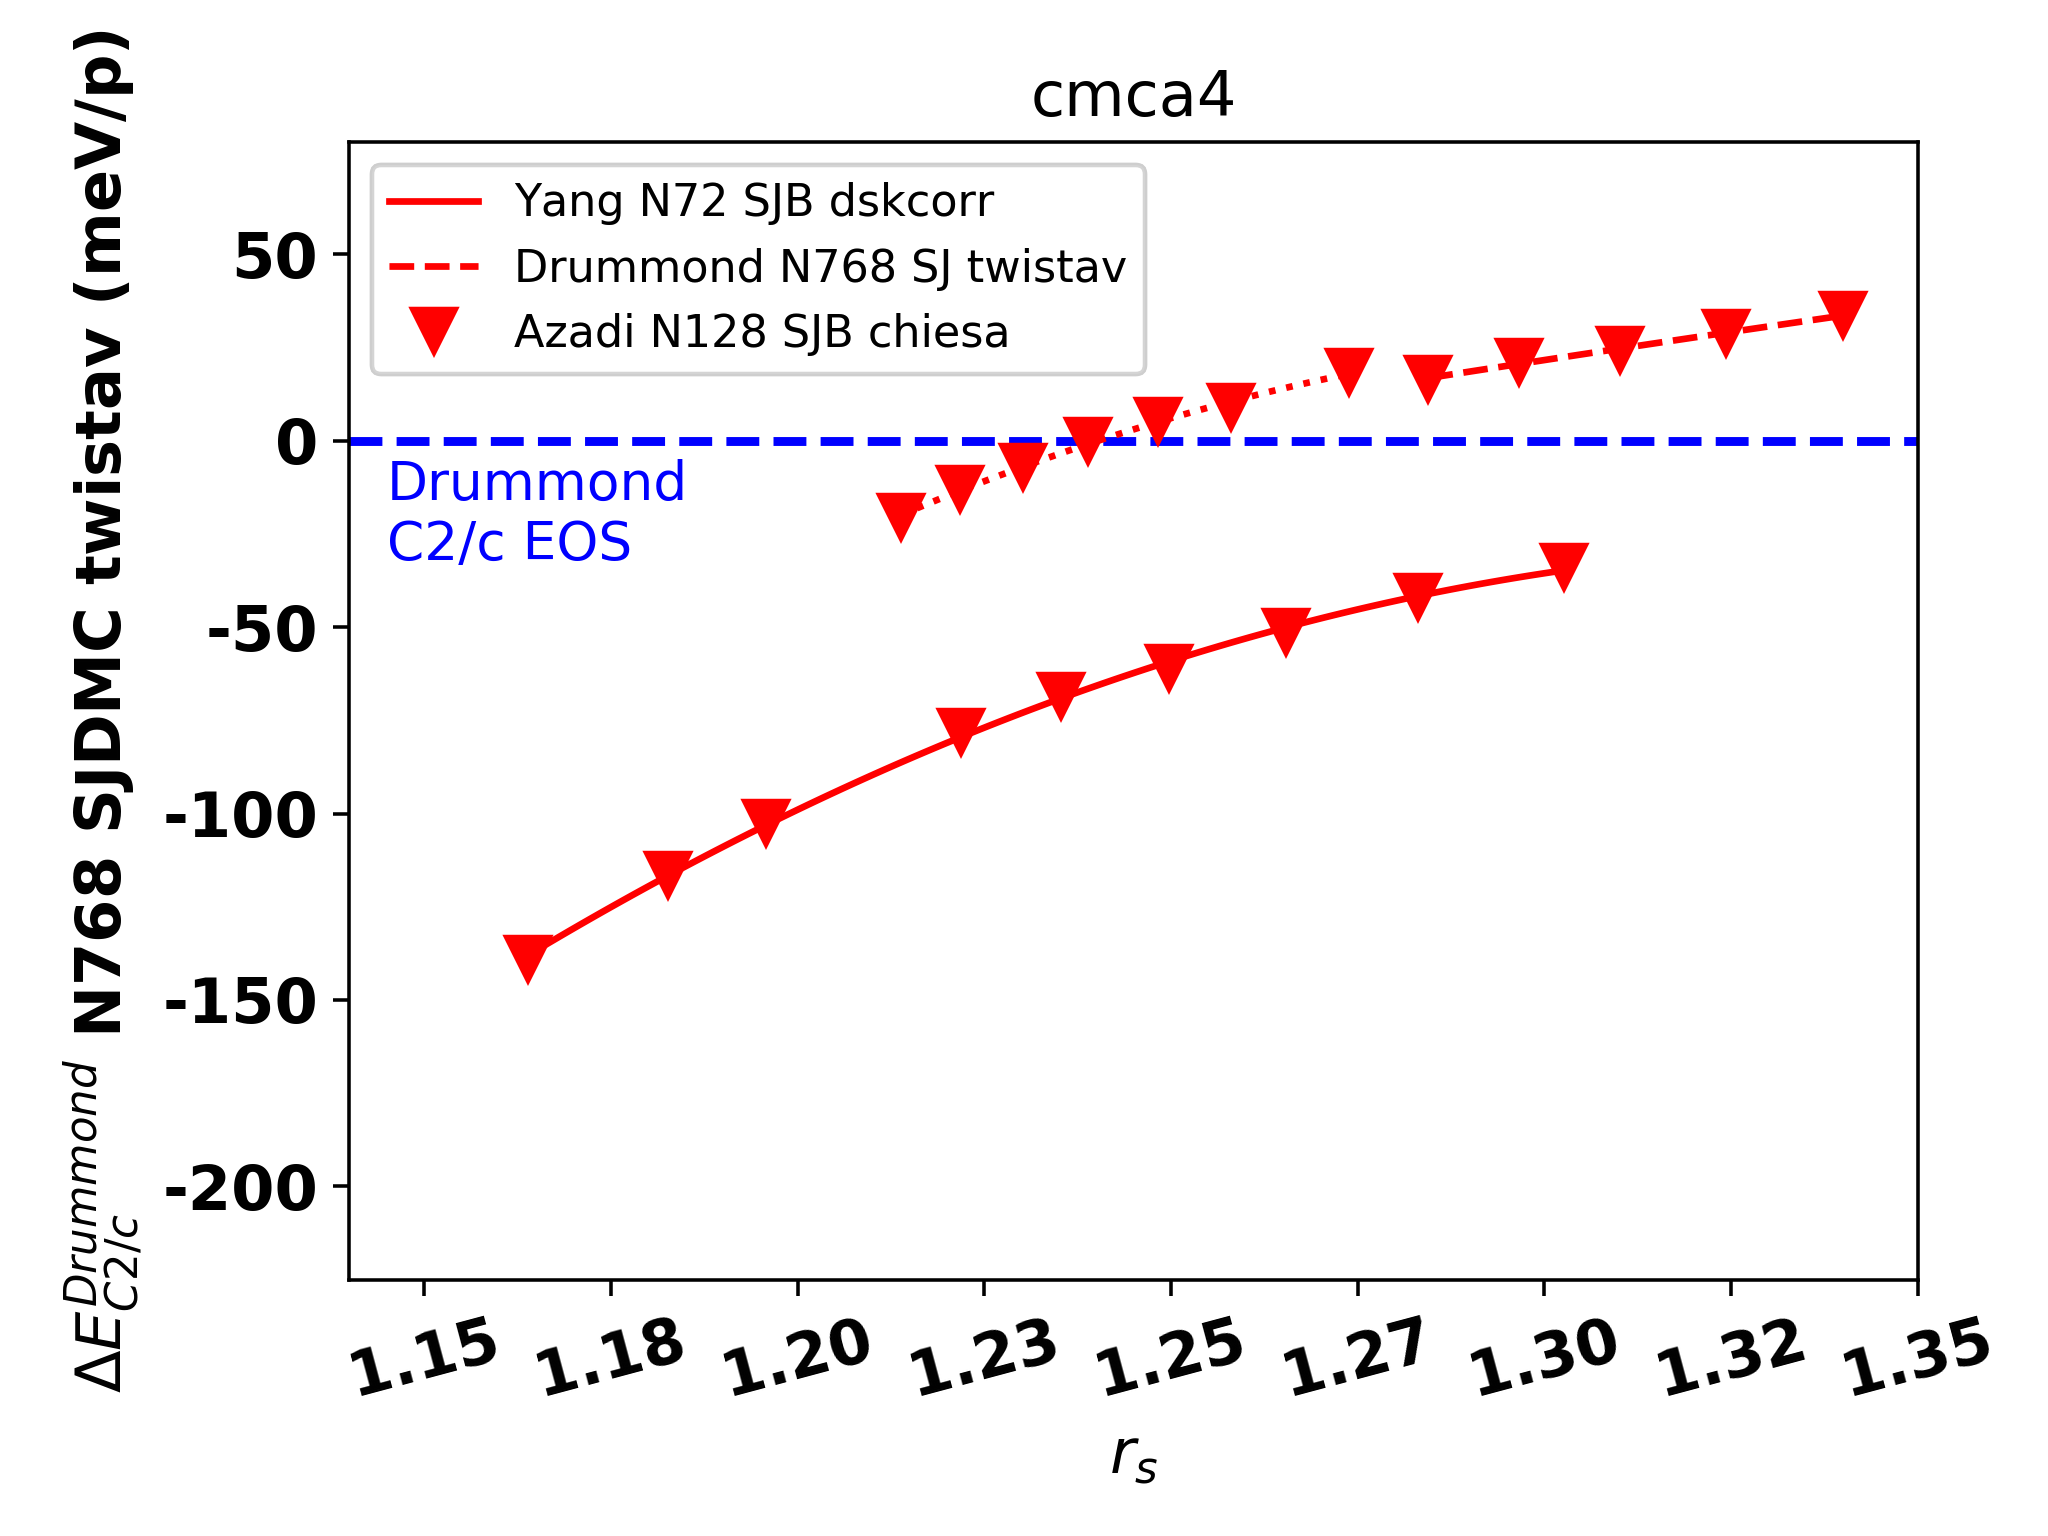
\includegraphics[width=\columnwidth]{006b_cmca4_step0}
 (a) DMC data.%\label{fig:static-cmca4-yang-drummond-azadi-data}
\end{minipage}
%\begin{subfigure}{0.48\textwidth}
%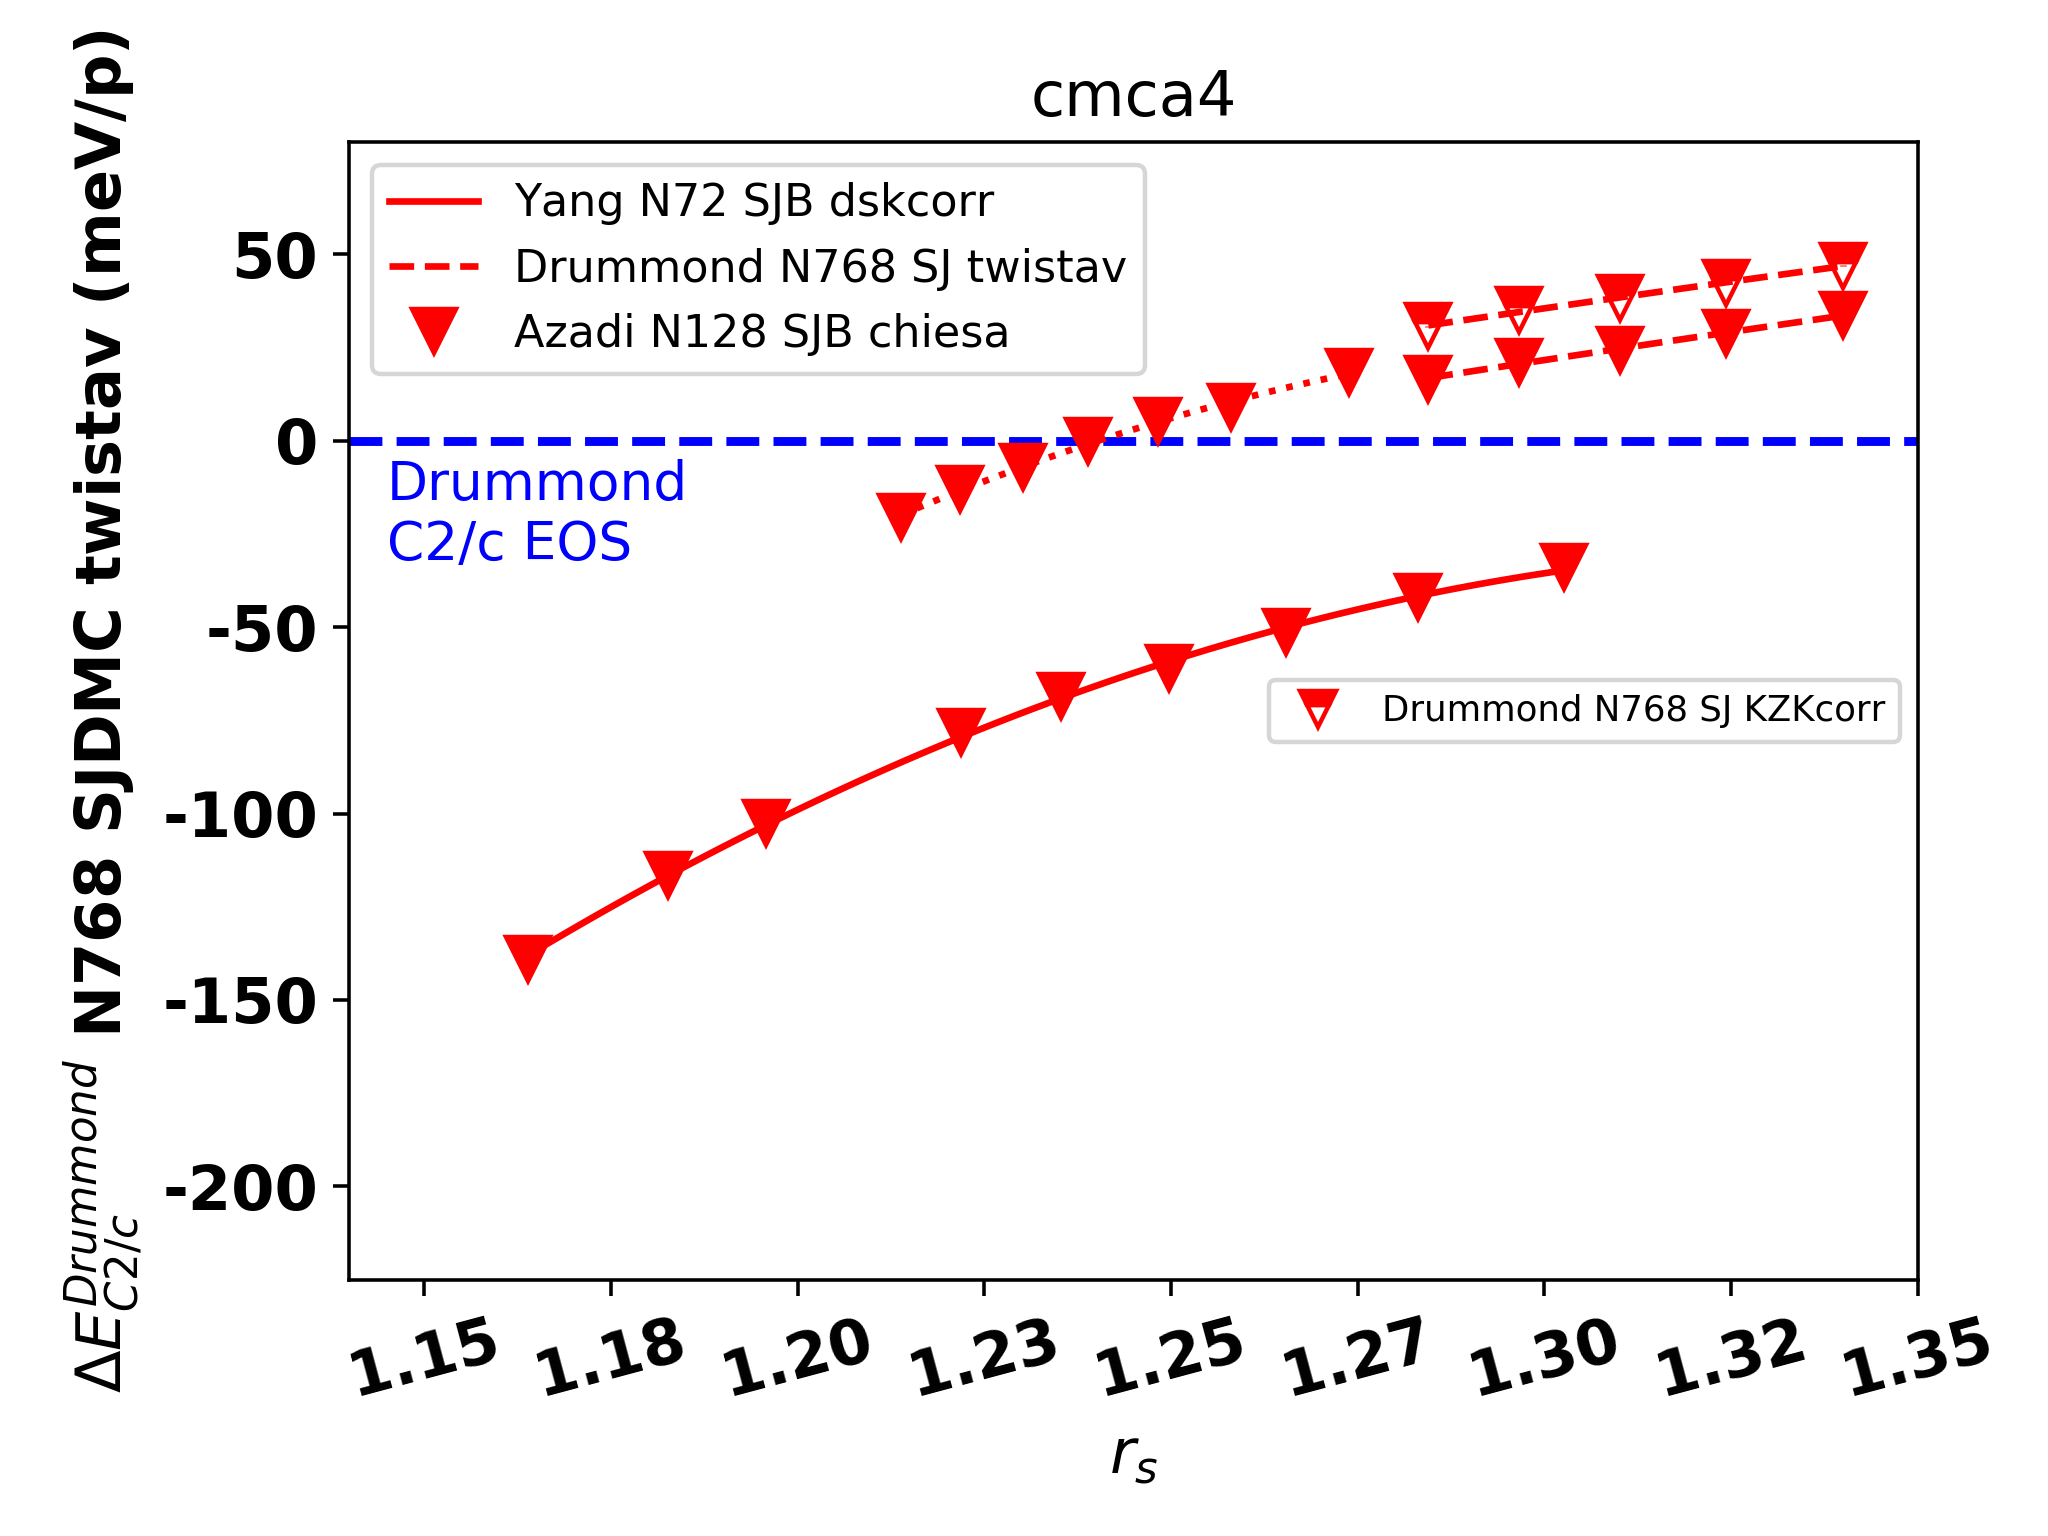
\includegraphics[scale=0.48]{figures/cmca4/006b_cmca4_step1}
%\caption{Add KZKcorr to Drummond.\label{fig:static-cmca4-yang-drummond-azadi-kzk}}
%\end{subfigure}
\begin{minipage}{0.48\textwidth}
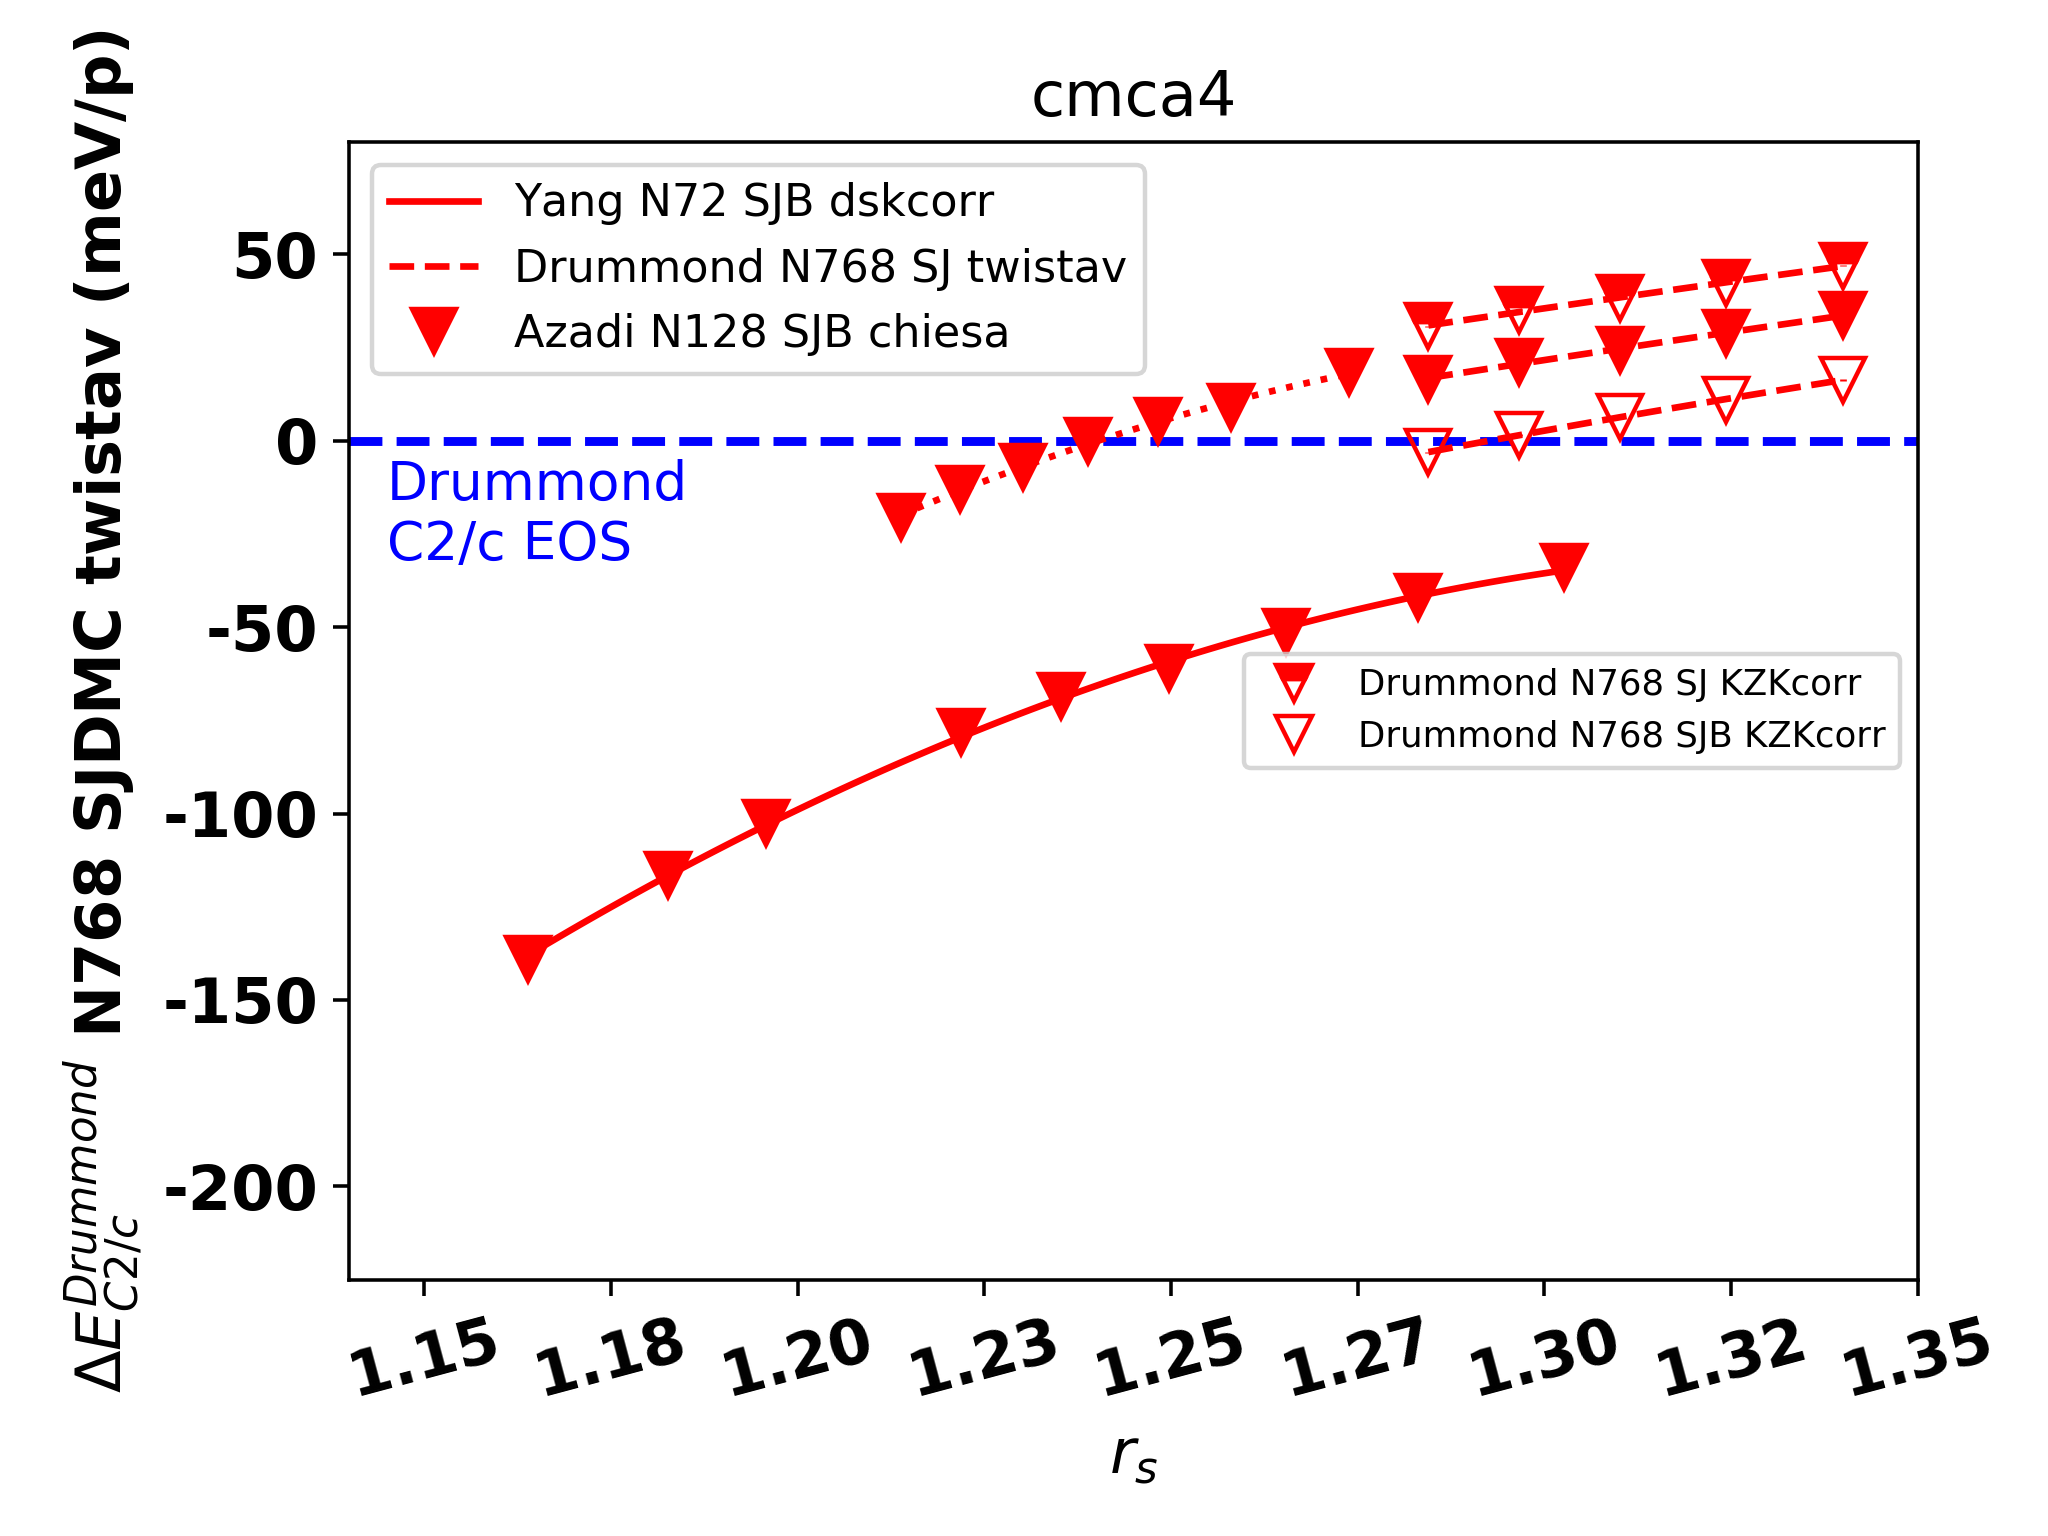
\includegraphics[scale=0.48]{006b_cmca4_step2}
(b) Add back flow to Drummond %\label{fig:static-cmca4-yang-drummond-azadi-sjb}
\end{minipage}
\caption{Cmca-4\label{fig:static-cmca4-yang-drummond-azadi}}
\end{figure}

\subsection{Molecular Candidate Cmca-12}

Three sets of data are shown in Fig.~\ref{fig:static-cmca12-yang-drummond-azadi-data}. The right-filled triangles connected by a dashed line near -100 meV/p at low density ($r_s>1.27$) are Drummond's N96 SJ twistav results. The right-filled triangles connected by a dotted line are Azadi's N96 SJB twistav results. The solid triangles connected by a solid line are my N72 SJB dskcorr results. At $r_s=1.30$ my SBJ dskcorr energy is lower than Drummond's SBJ KZKcorr energy by \textbf{41 meV/p}.

In Fig.~\ref{fig:static-cmca12-yang-drummond-azadi-kzk}, Drummond's N768 SJB KZKcorr results are added as open triangles.

Azadi's N96 SJB twistav energies are higher than Drummond's N96 SJ twistav. This is surprising. No FS correction scheme beyond twist averaging is applied to either data set. Both Azadi and Drummond use PBE geometry, so their structures should agree. I expect Azadi's SJB energy to be lower than Drummond's SJ energy due to the inclusion of back flow. However, actual data indicate the contrary.

\begin{figure}[h]
\begin{minipage}{0.48\textwidth}
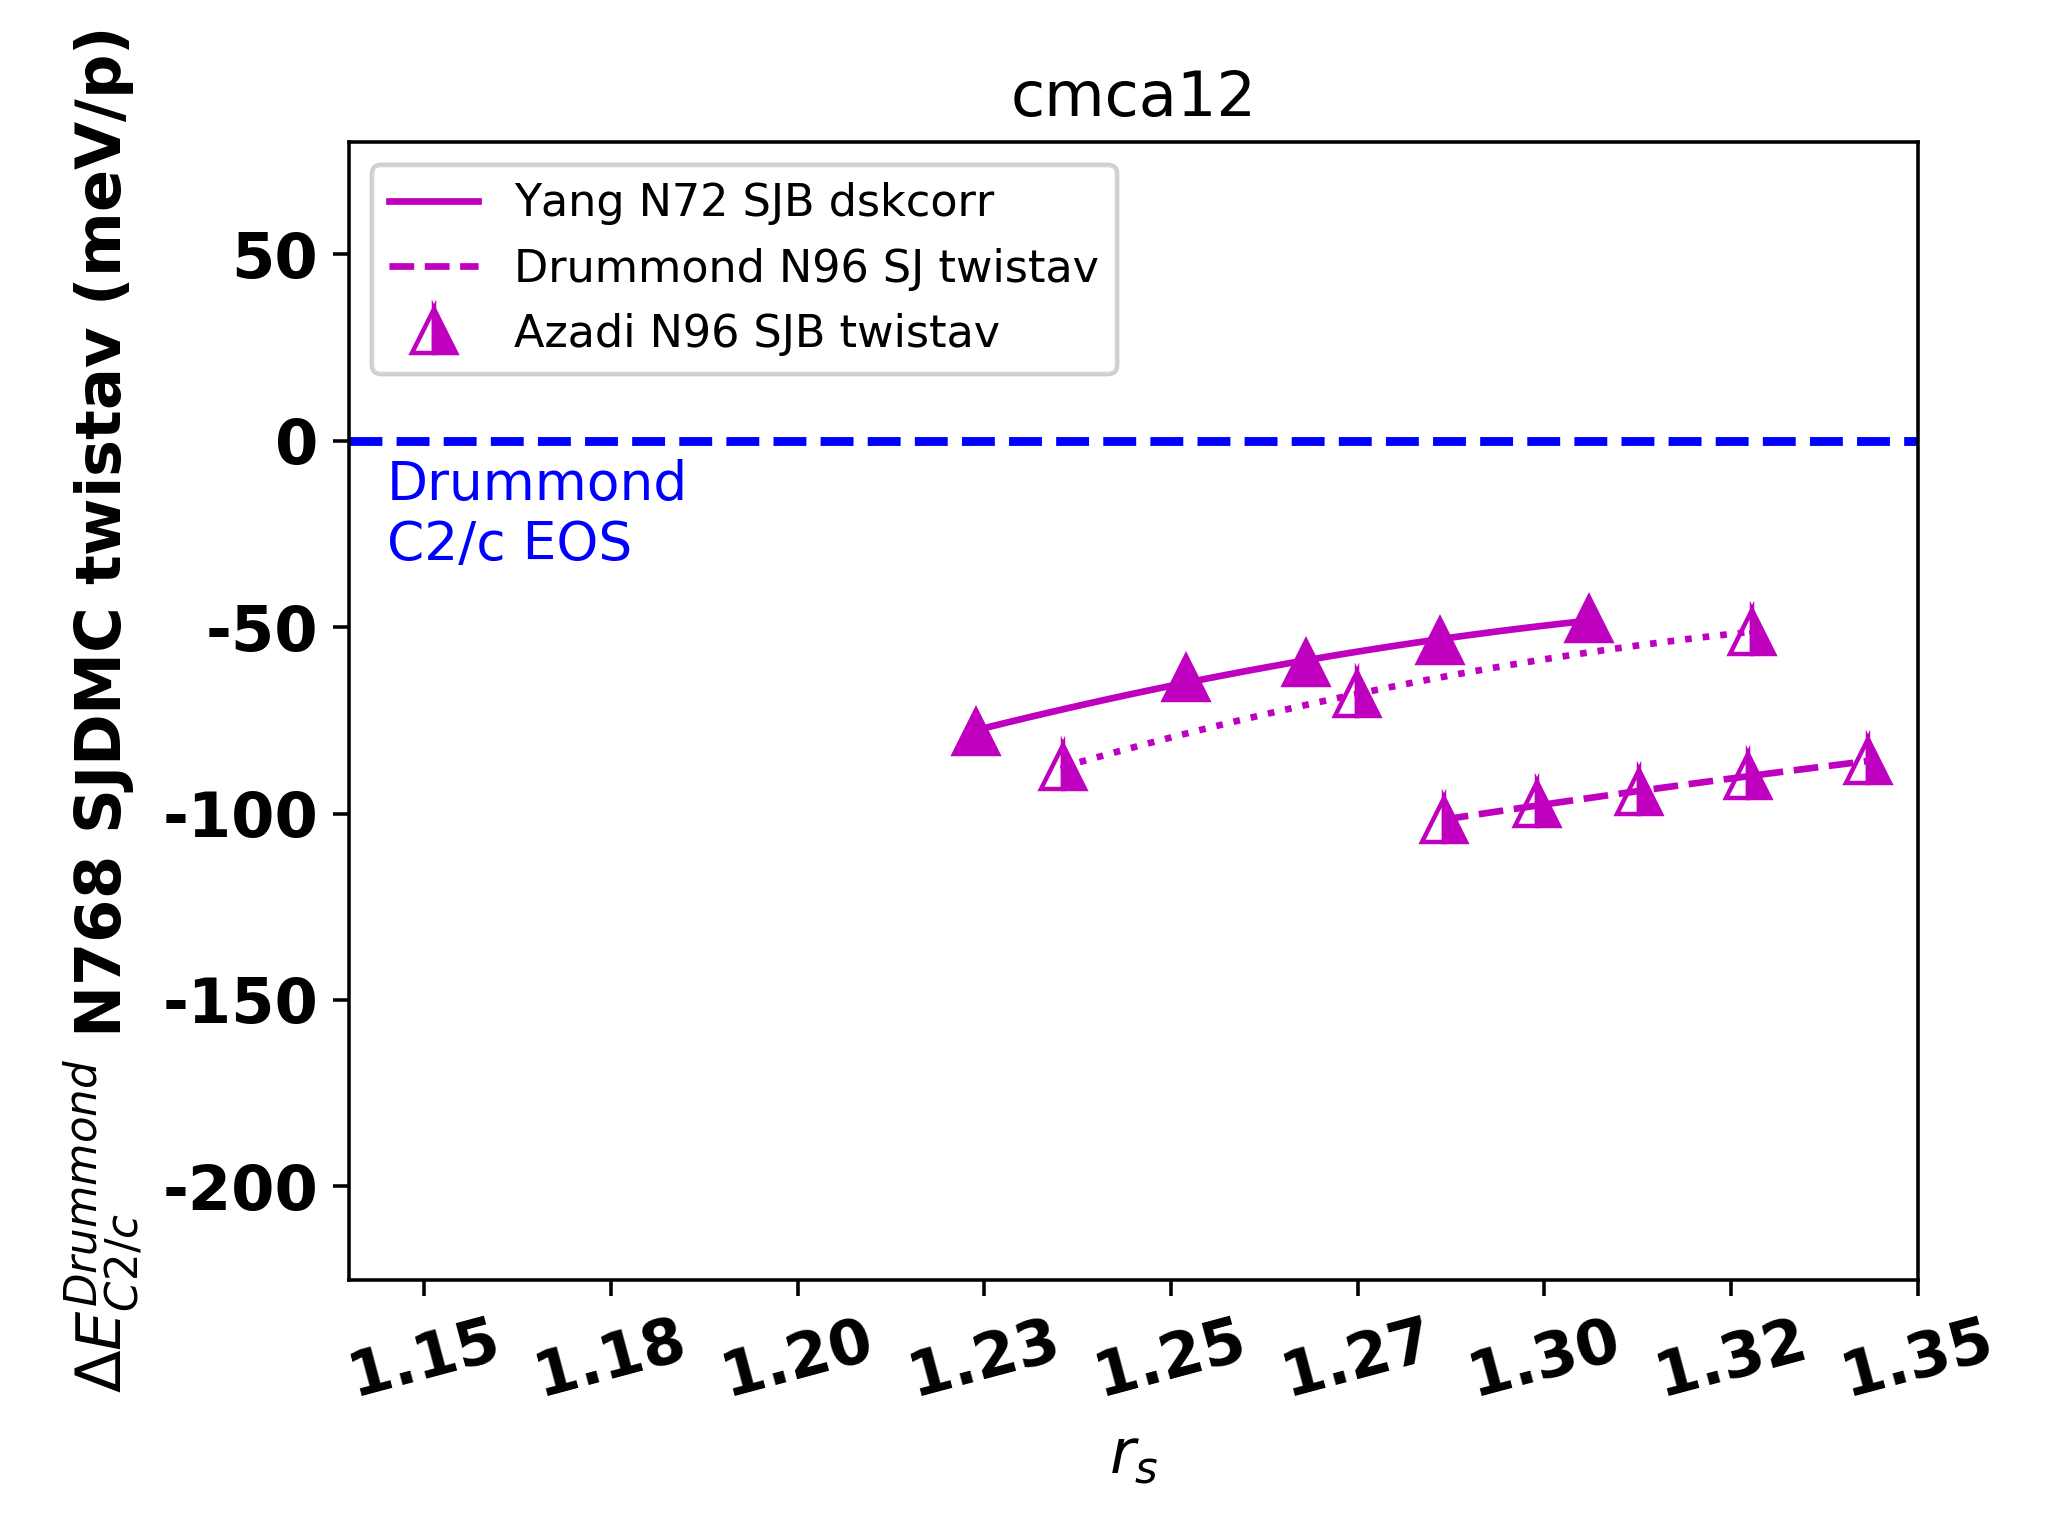
\includegraphics[width=\columnwidth]{006b_cmca12_step0}
%\caption{DMC data.\label{fig:static-cmca12-yang-drummond-azadi-data}}
\end{minipage}
\begin{minipage}{0.48\textwidth}
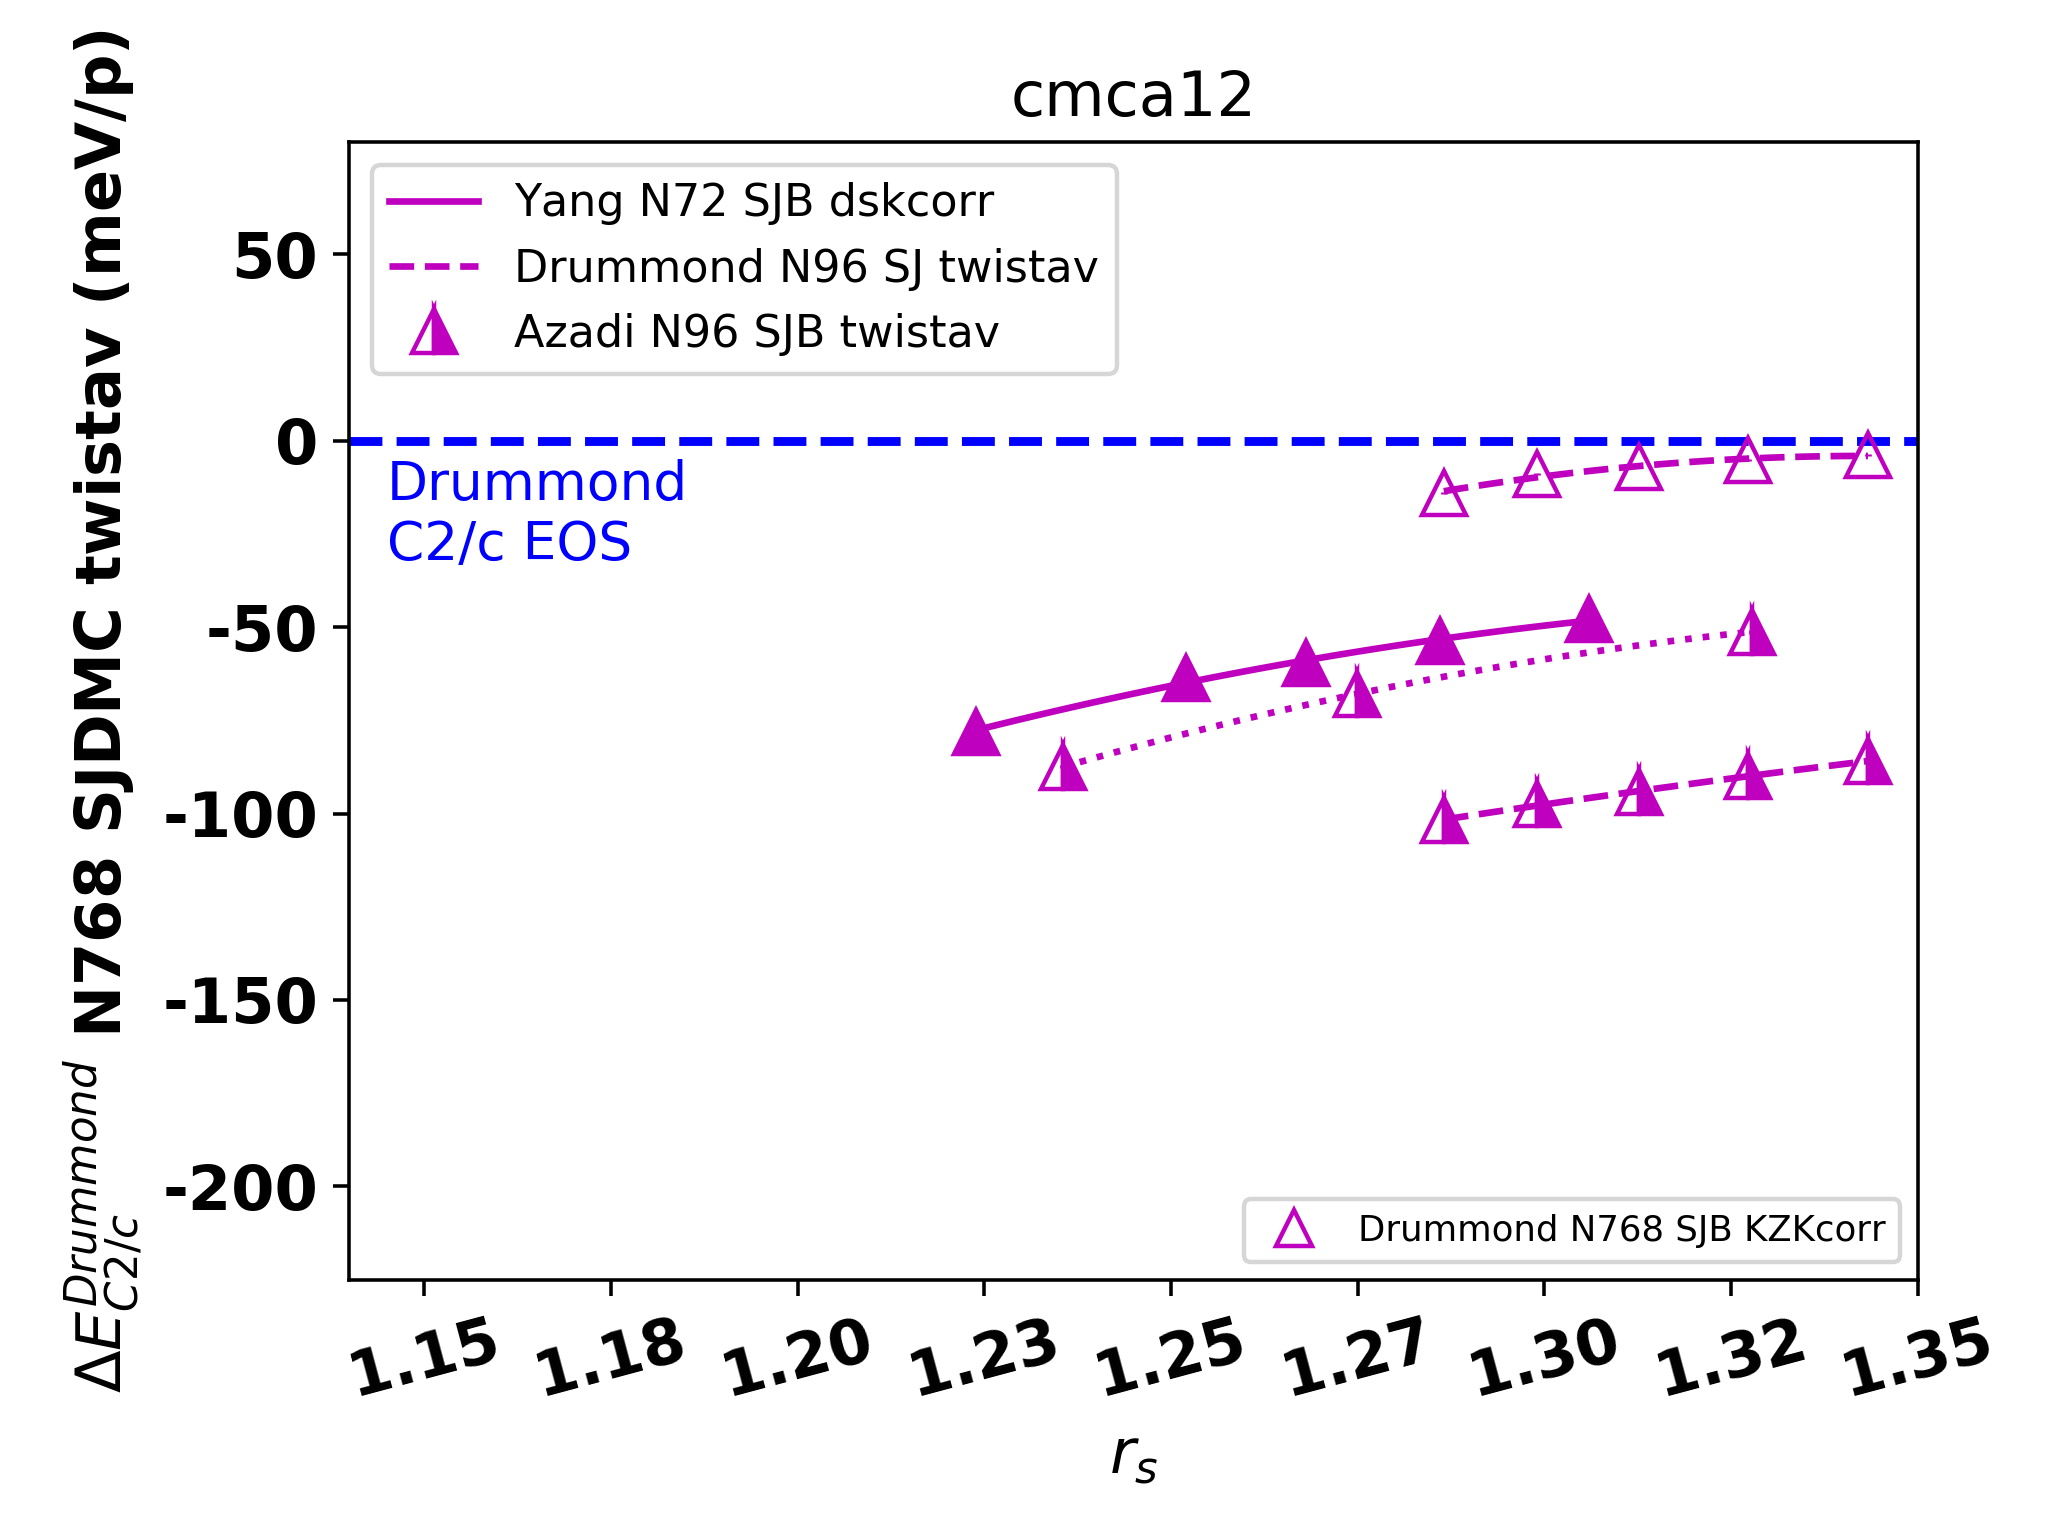
\includegraphics[width=\columnwidth]{006b_cmca12_step1}
%\caption{DMC data.\label{fig:static-cmca12-yang-drummond-azadi-kzk}}
\end{minipage}
\caption{Cmca-12\label{fig:static-cmca12-yang-drummond-azadi}}
\end{figure}

